Here are the differential cross-section plots for various xF bins.

% --- Plot for xF Bin 0 ---
\begin{figure}[p] % 'p' suggests placing the figure on a separate page
\centering
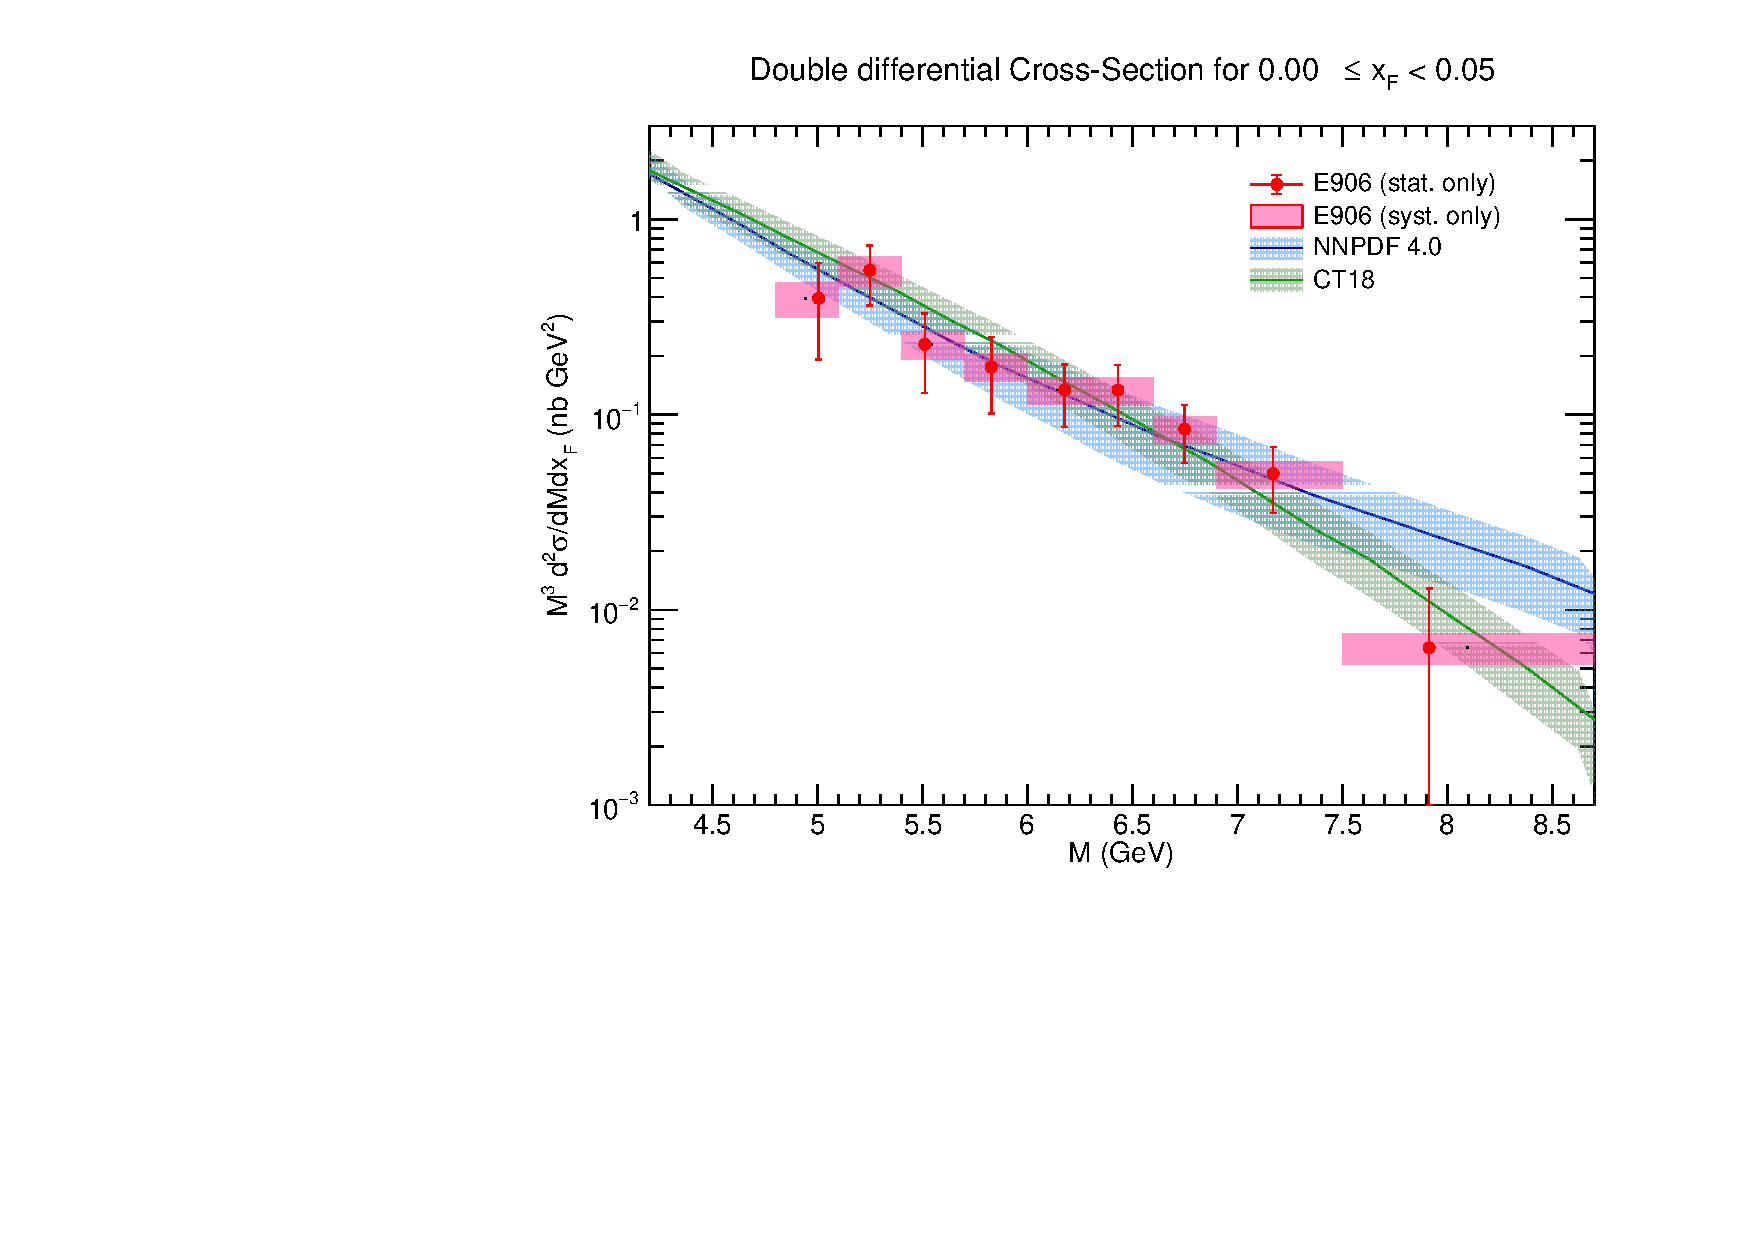
\includegraphics[width=0.9\textwidth]{./XSecPlots/LH2_0_roofit.pdf}
\caption{Plot for xF bin 0.}
\end{figure}
\clearpage

% --- Plot for xF Bin 1 ---
\begin{figure}[p]
\centering
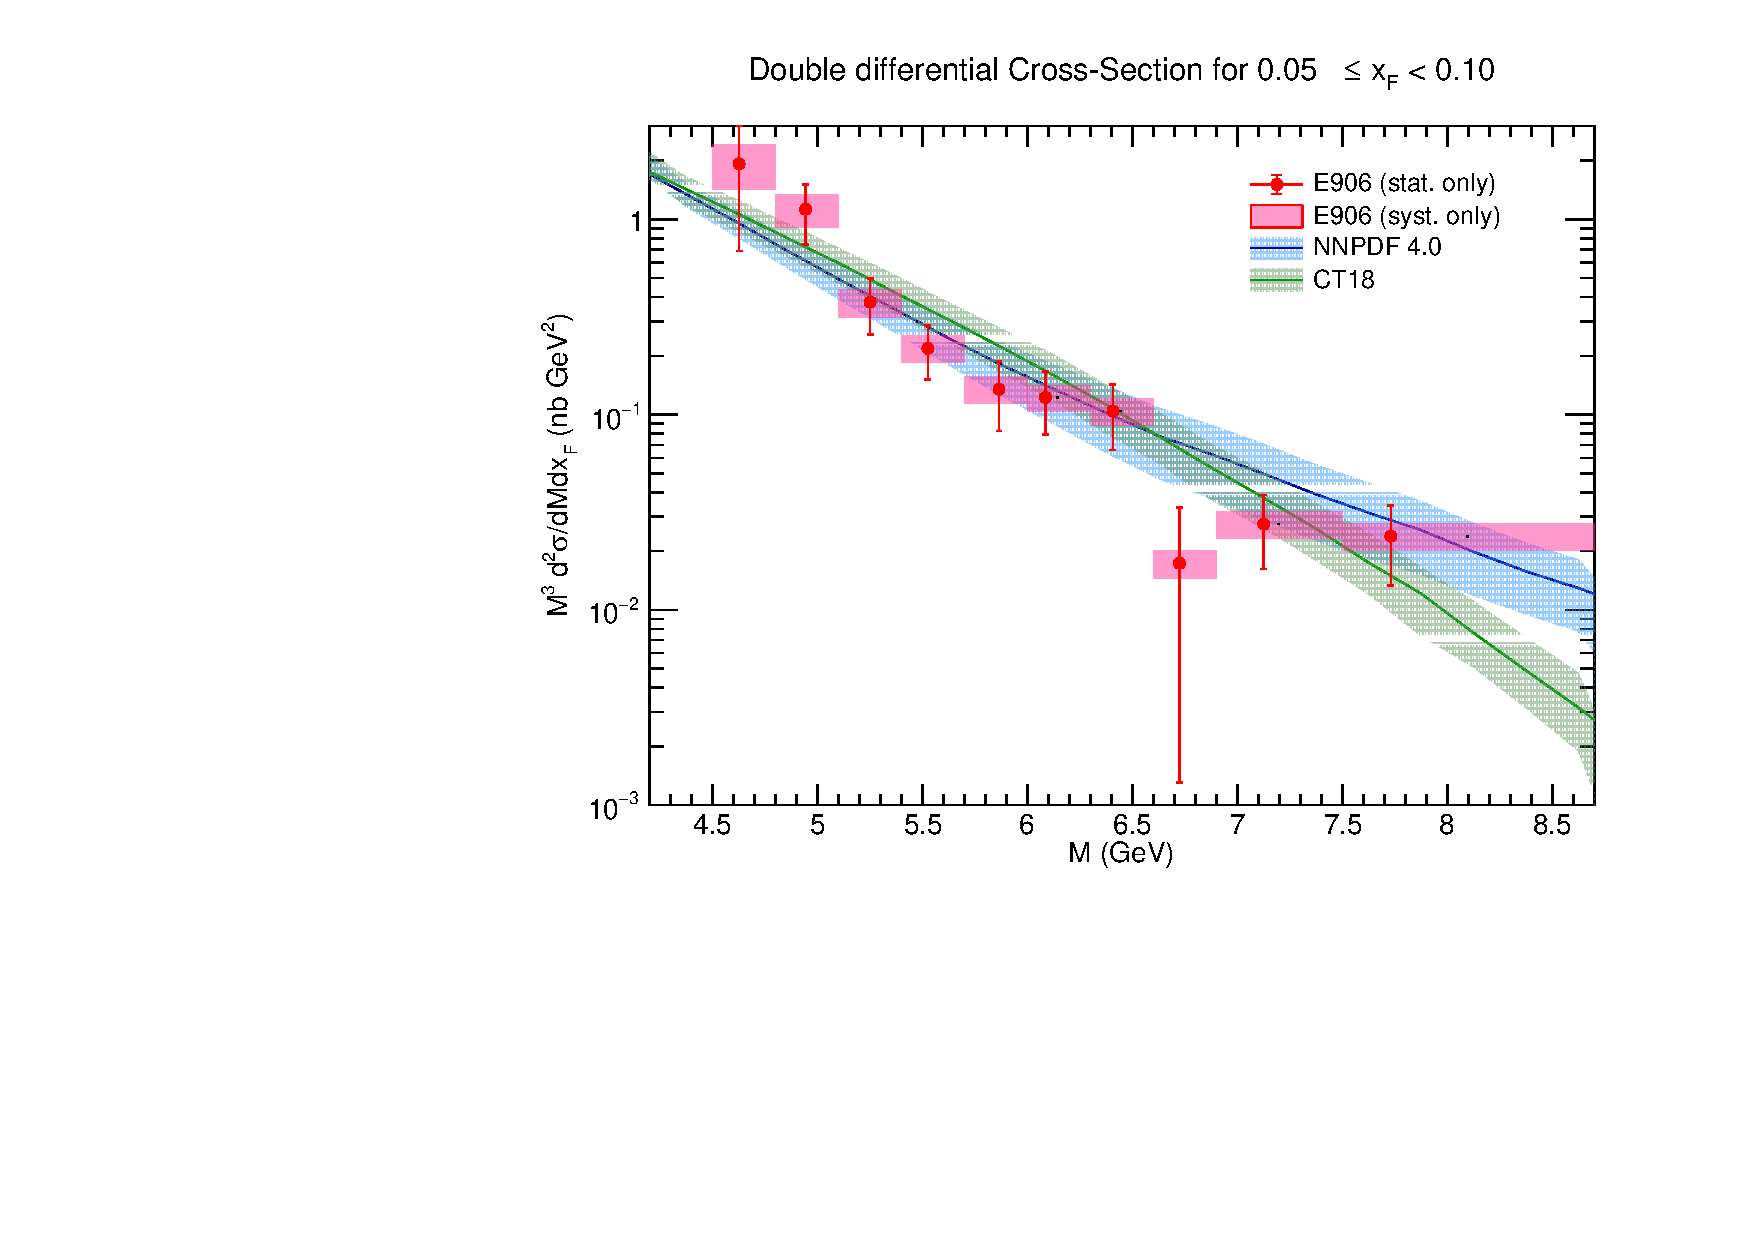
\includegraphics[width=0.9\textwidth]{./XSecPlots/LH2_1_roofit.pdf}
\caption{Plot for xF bin 1.}
\end{figure}
\clearpage

% --- Plot for xF Bin 2 ---
\begin{figure}[p]
\centering
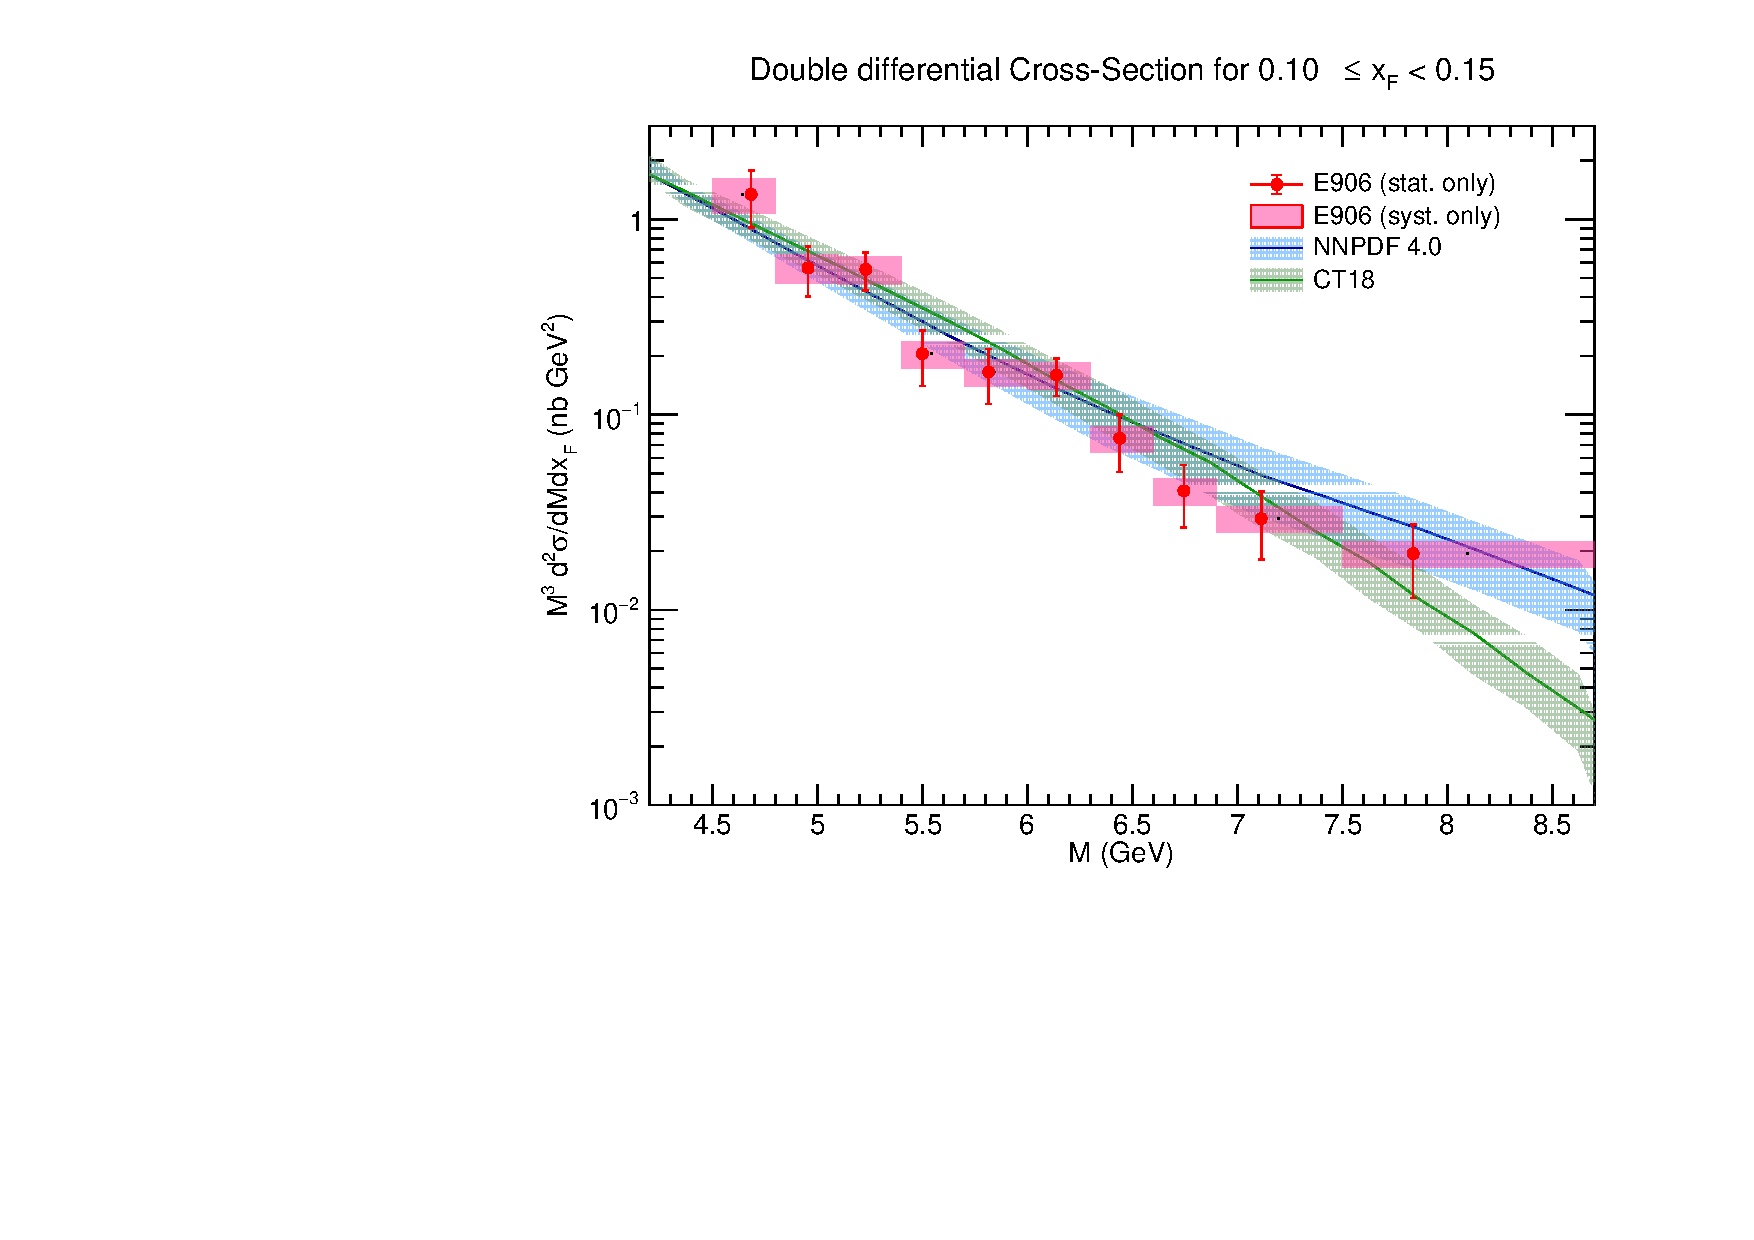
\includegraphics[width=0.9\textwidth]{./XSecPlots/LH2_2_roofit.pdf}
\caption{Plot for xF bin 2.}
\end{figure}
\clearpage

% --- Plot for xF Bin 3 ---
\begin{figure}[p]
\centering
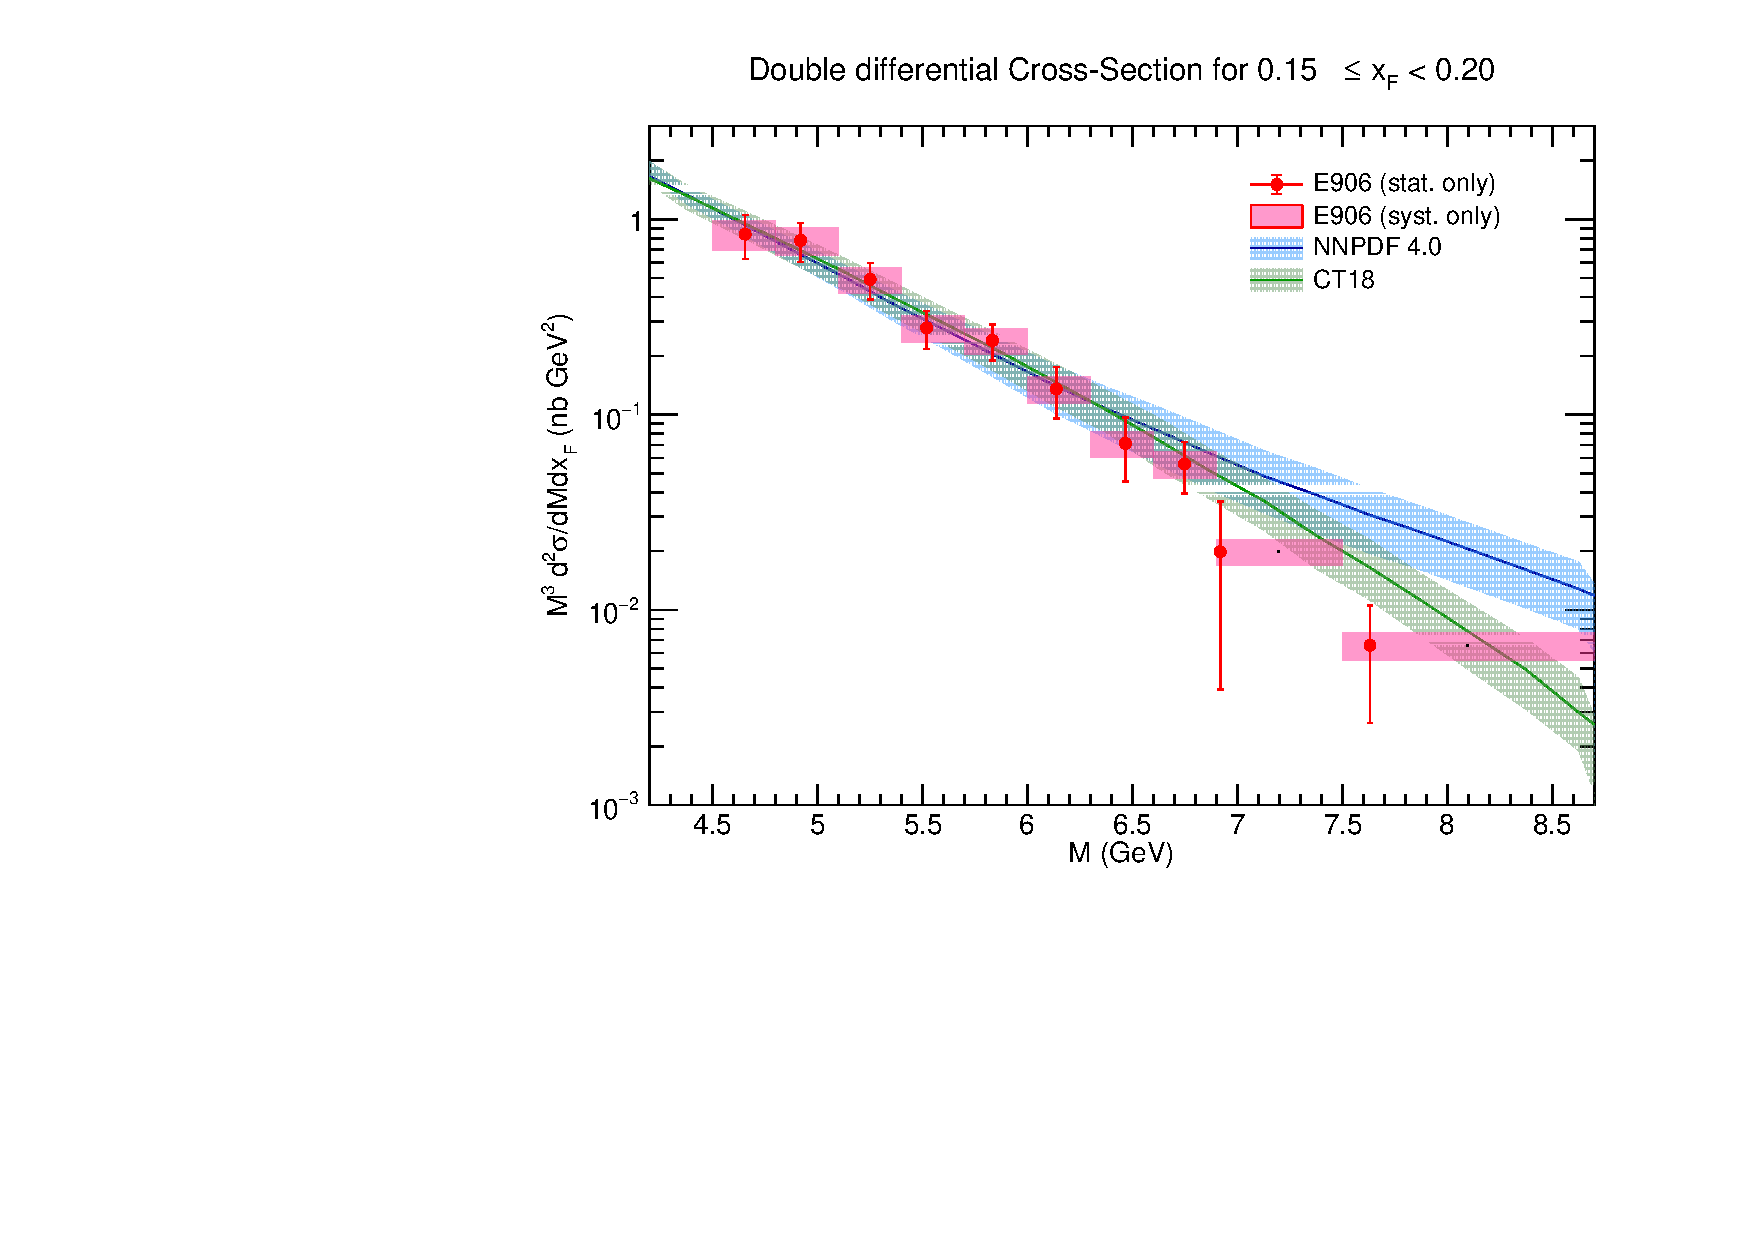
\includegraphics[width=0.9\textwidth]{./XSecPlots/LH2_3_roofit.pdf}
\caption{Plot for xF bin 3.}
\end{figure}
\clearpage

% --- Plot for xF Bin 4 ---
\begin{figure}[p]
\centering
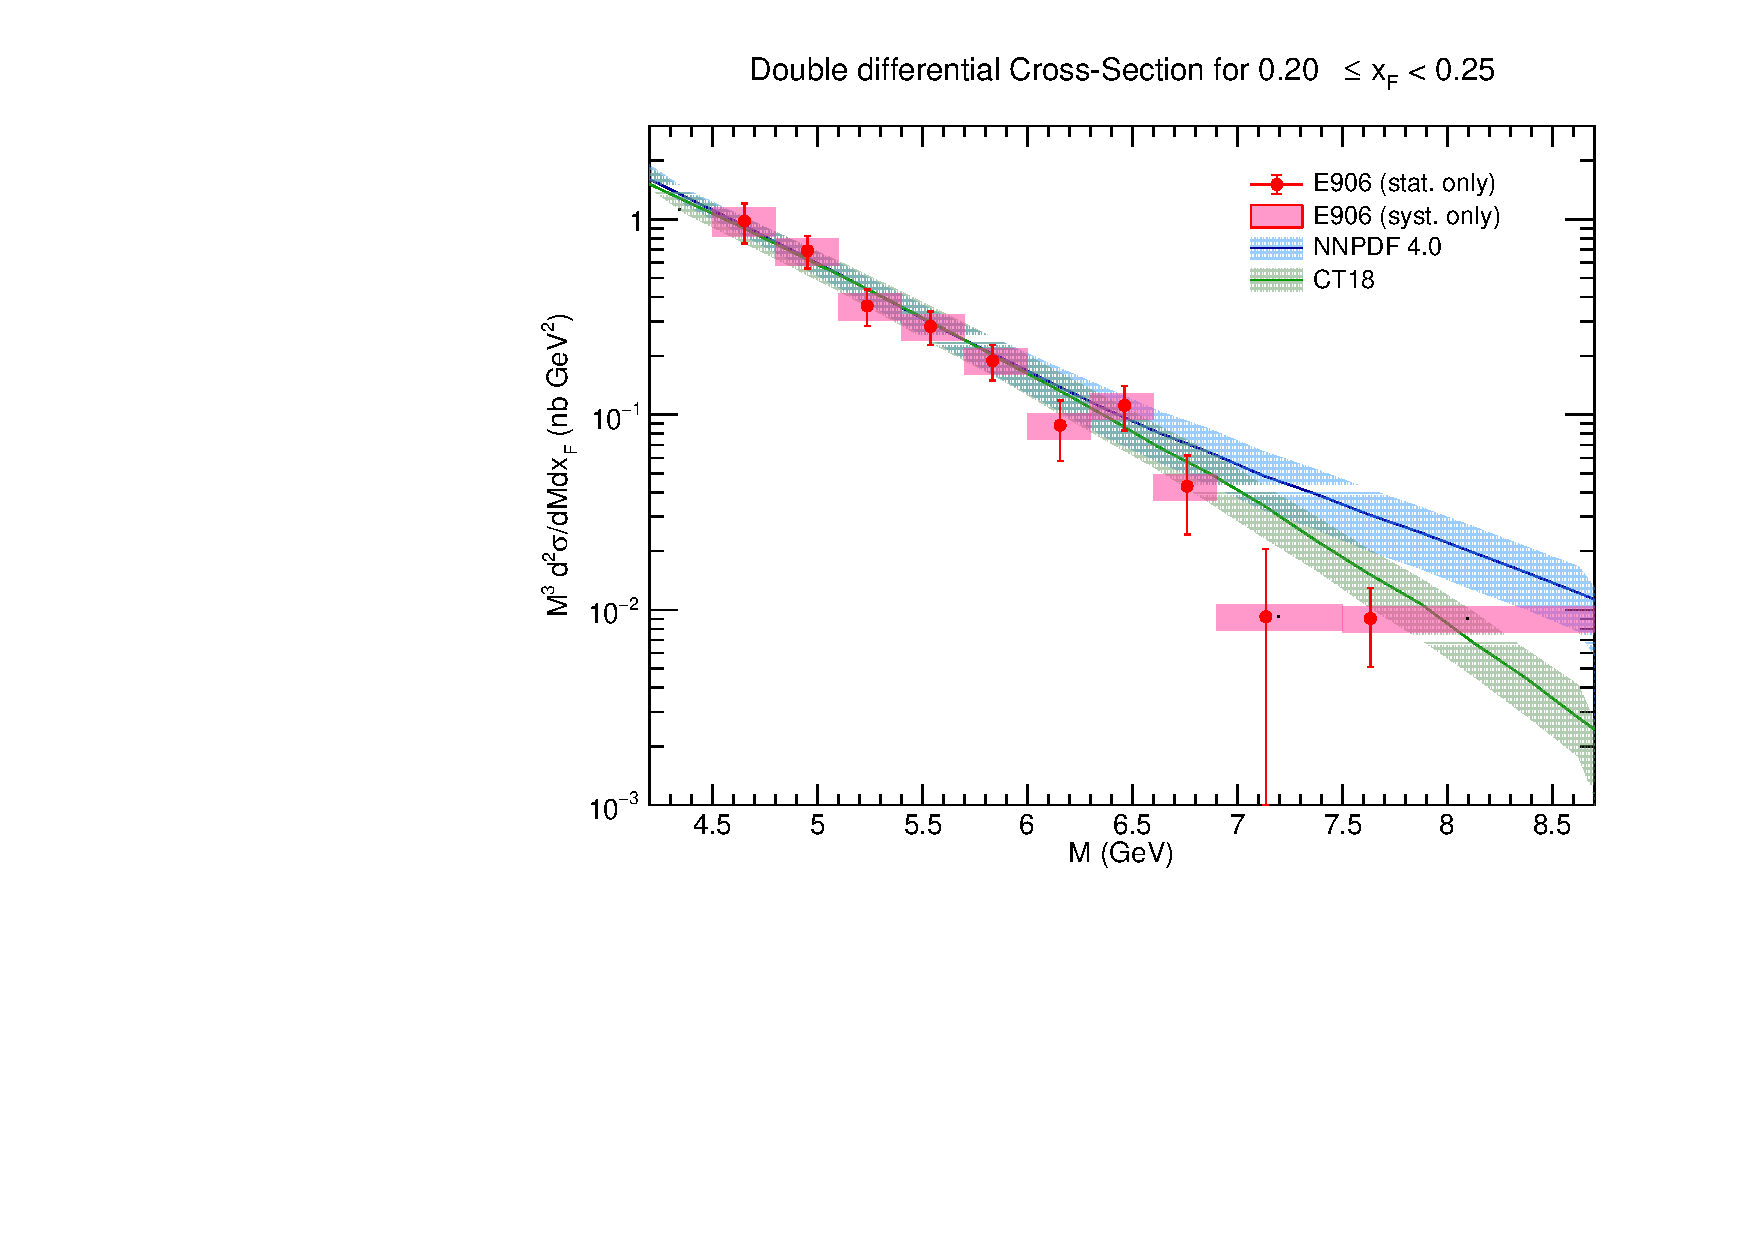
\includegraphics[width=0.9\textwidth]{./XSecPlots/LH2_4_roofit.pdf}
\caption{Plot for xF bin 4.}
\end{figure}
\clearpage

% --- Plot for xF Bin 5 ---
\begin{figure}[p]
\centering
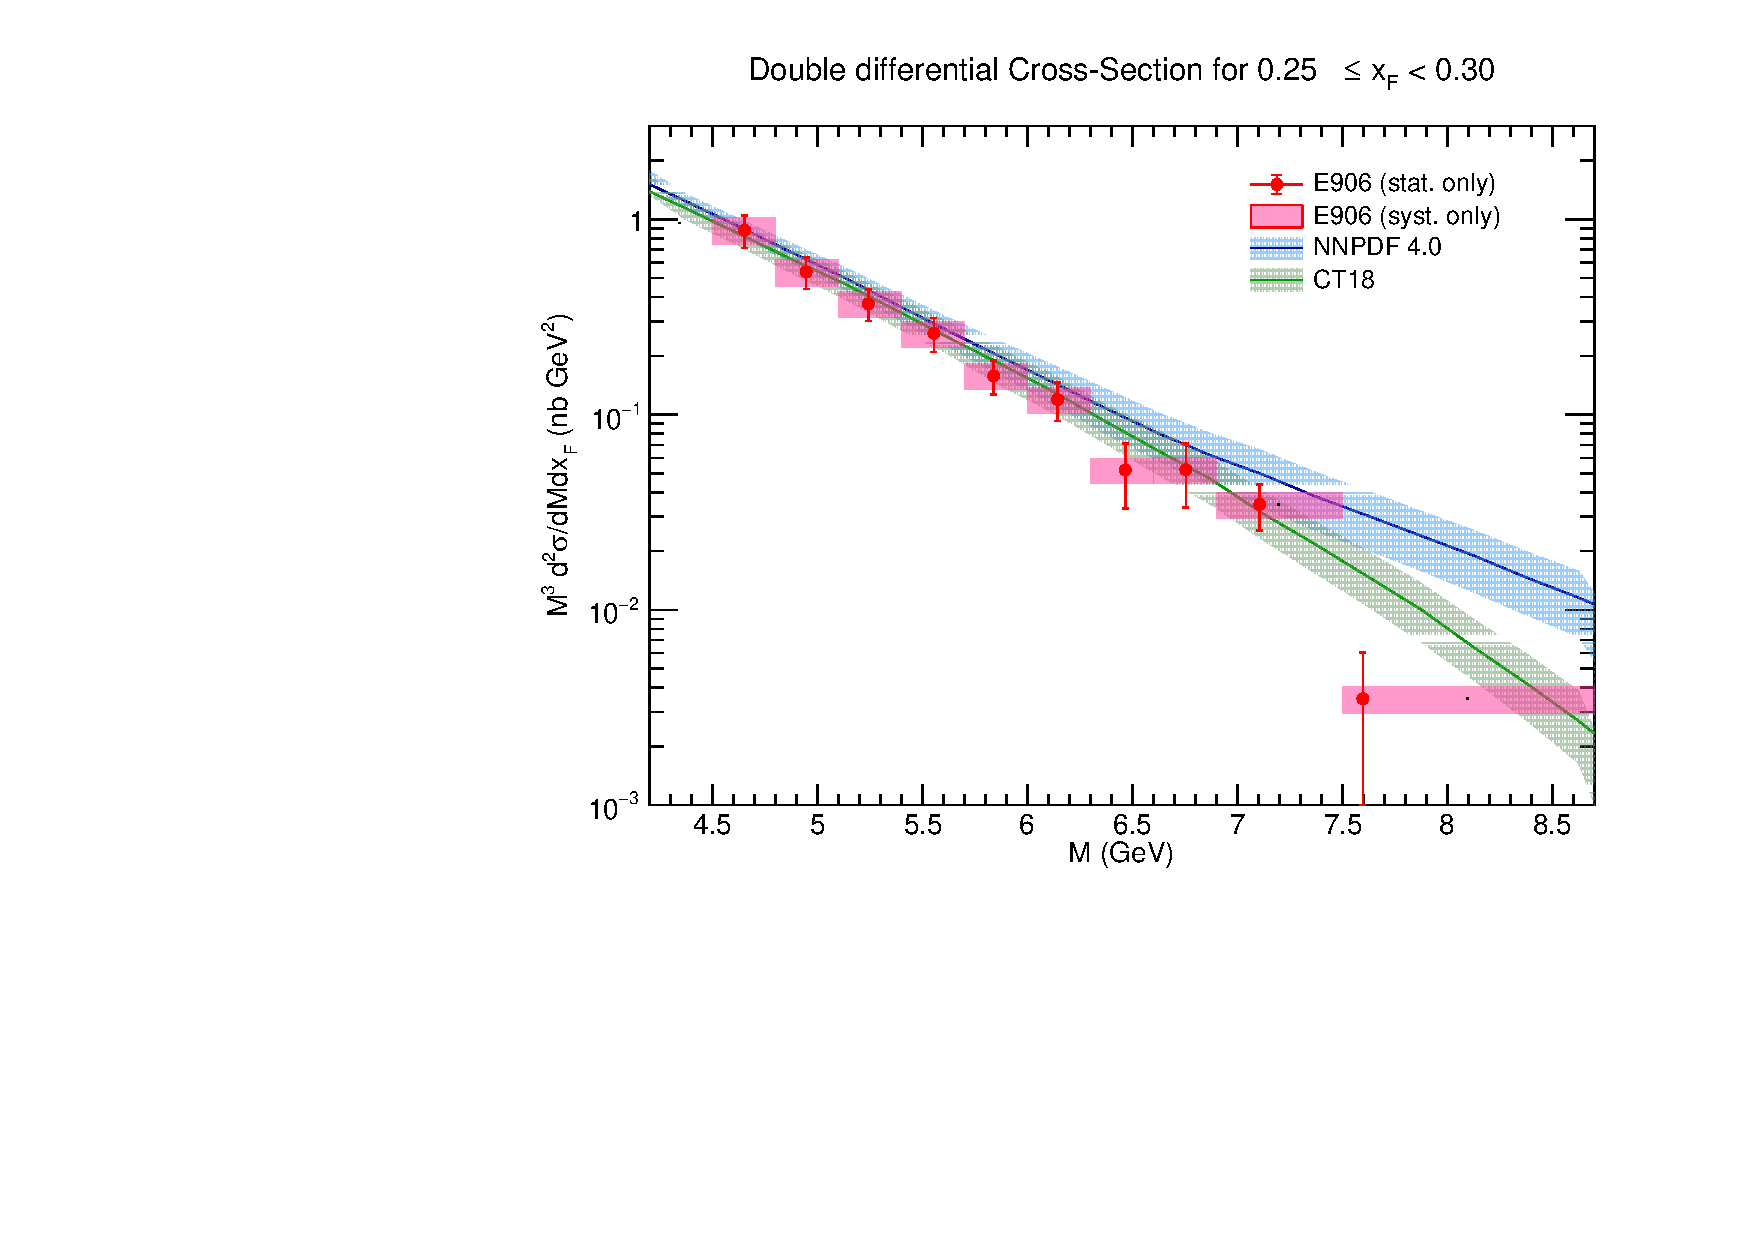
\includegraphics[width=0.9\textwidth]{./XSecPlots/LH2_5_roofit.pdf}
\caption{Plot for xF bin 5.}
\end{figure}
\clearpage

% --- Plot for xF Bin 6 ---
\begin{figure}[p]
\centering
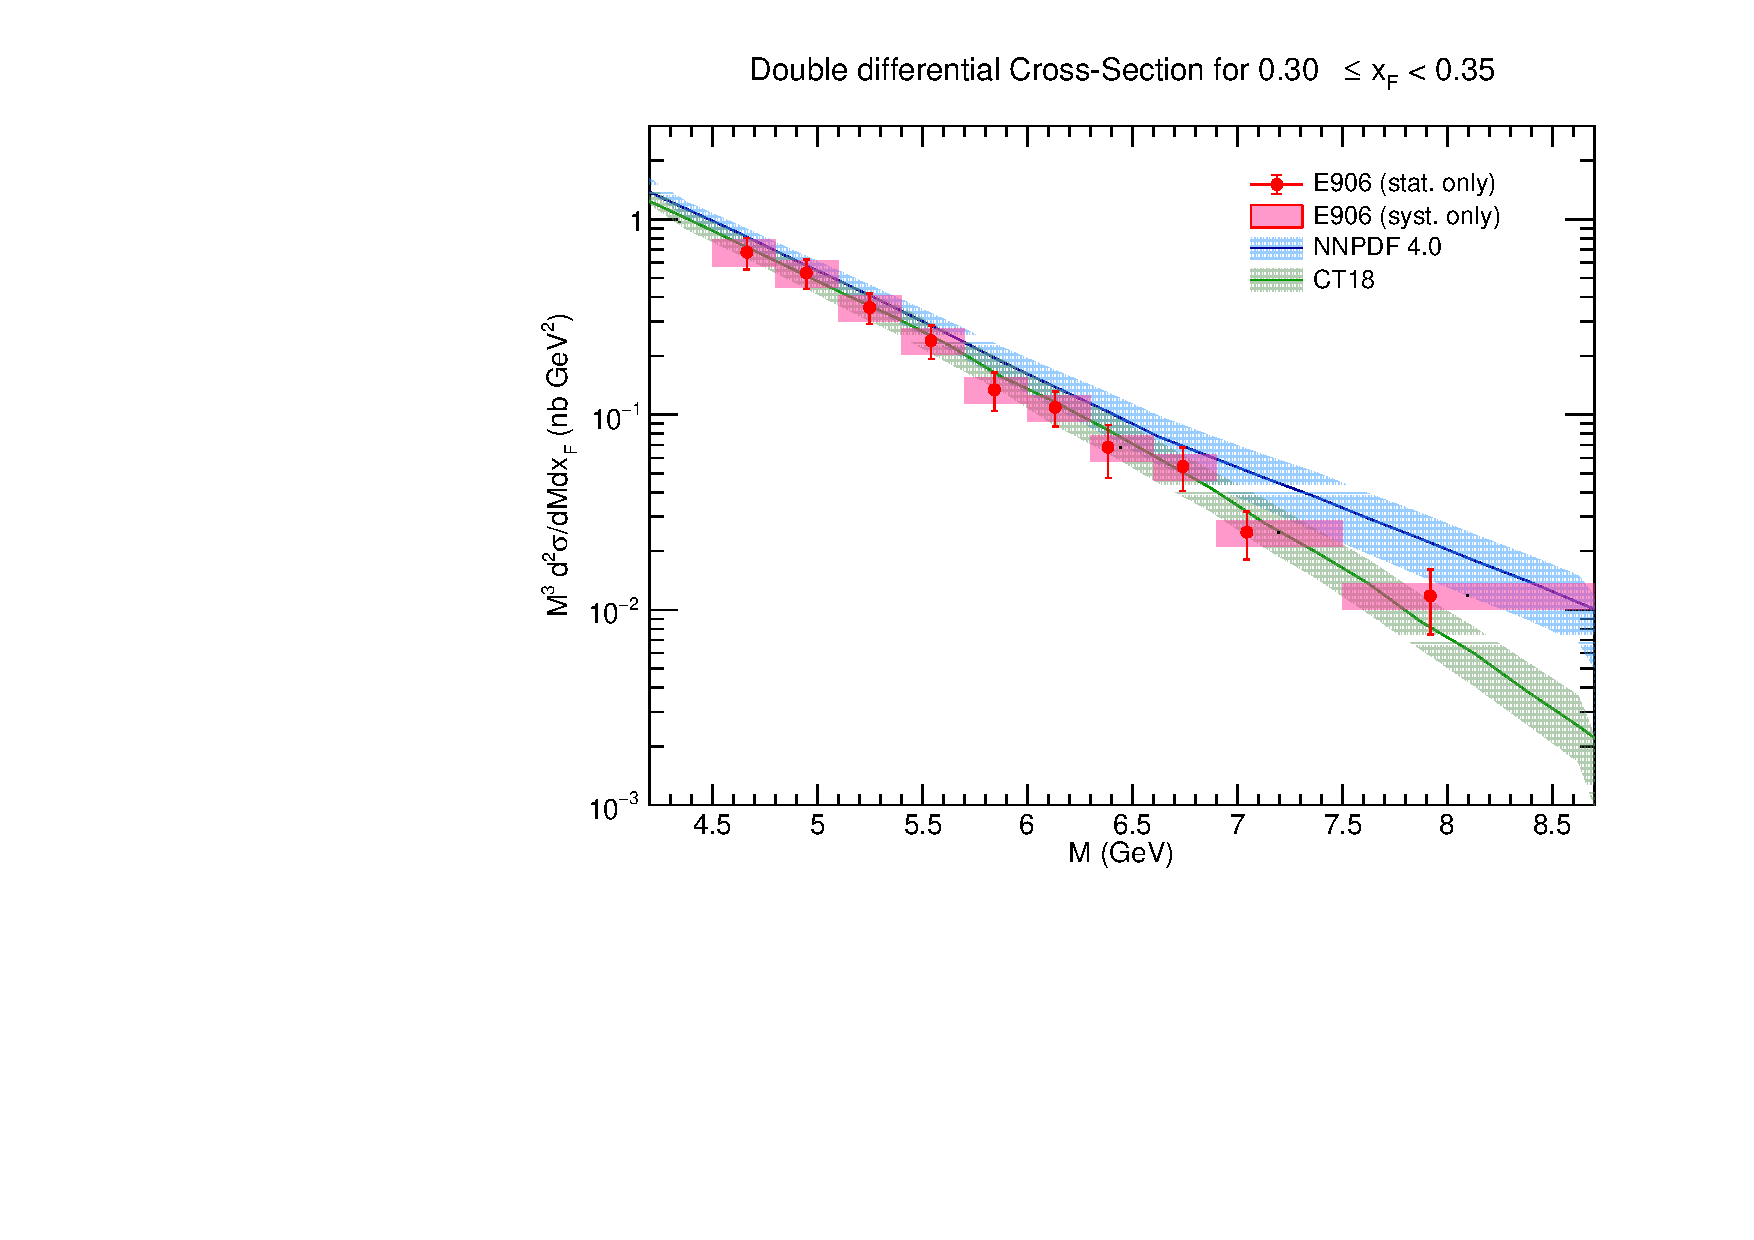
\includegraphics[width=0.9\textwidth]{./XSecPlots/LH2_6_roofit.pdf}
\caption{Plot for xF bin 6.}
\end{figure}
\clearpage

% --- Plot for xF Bin 7 ---
\begin{figure}[p]
\centering
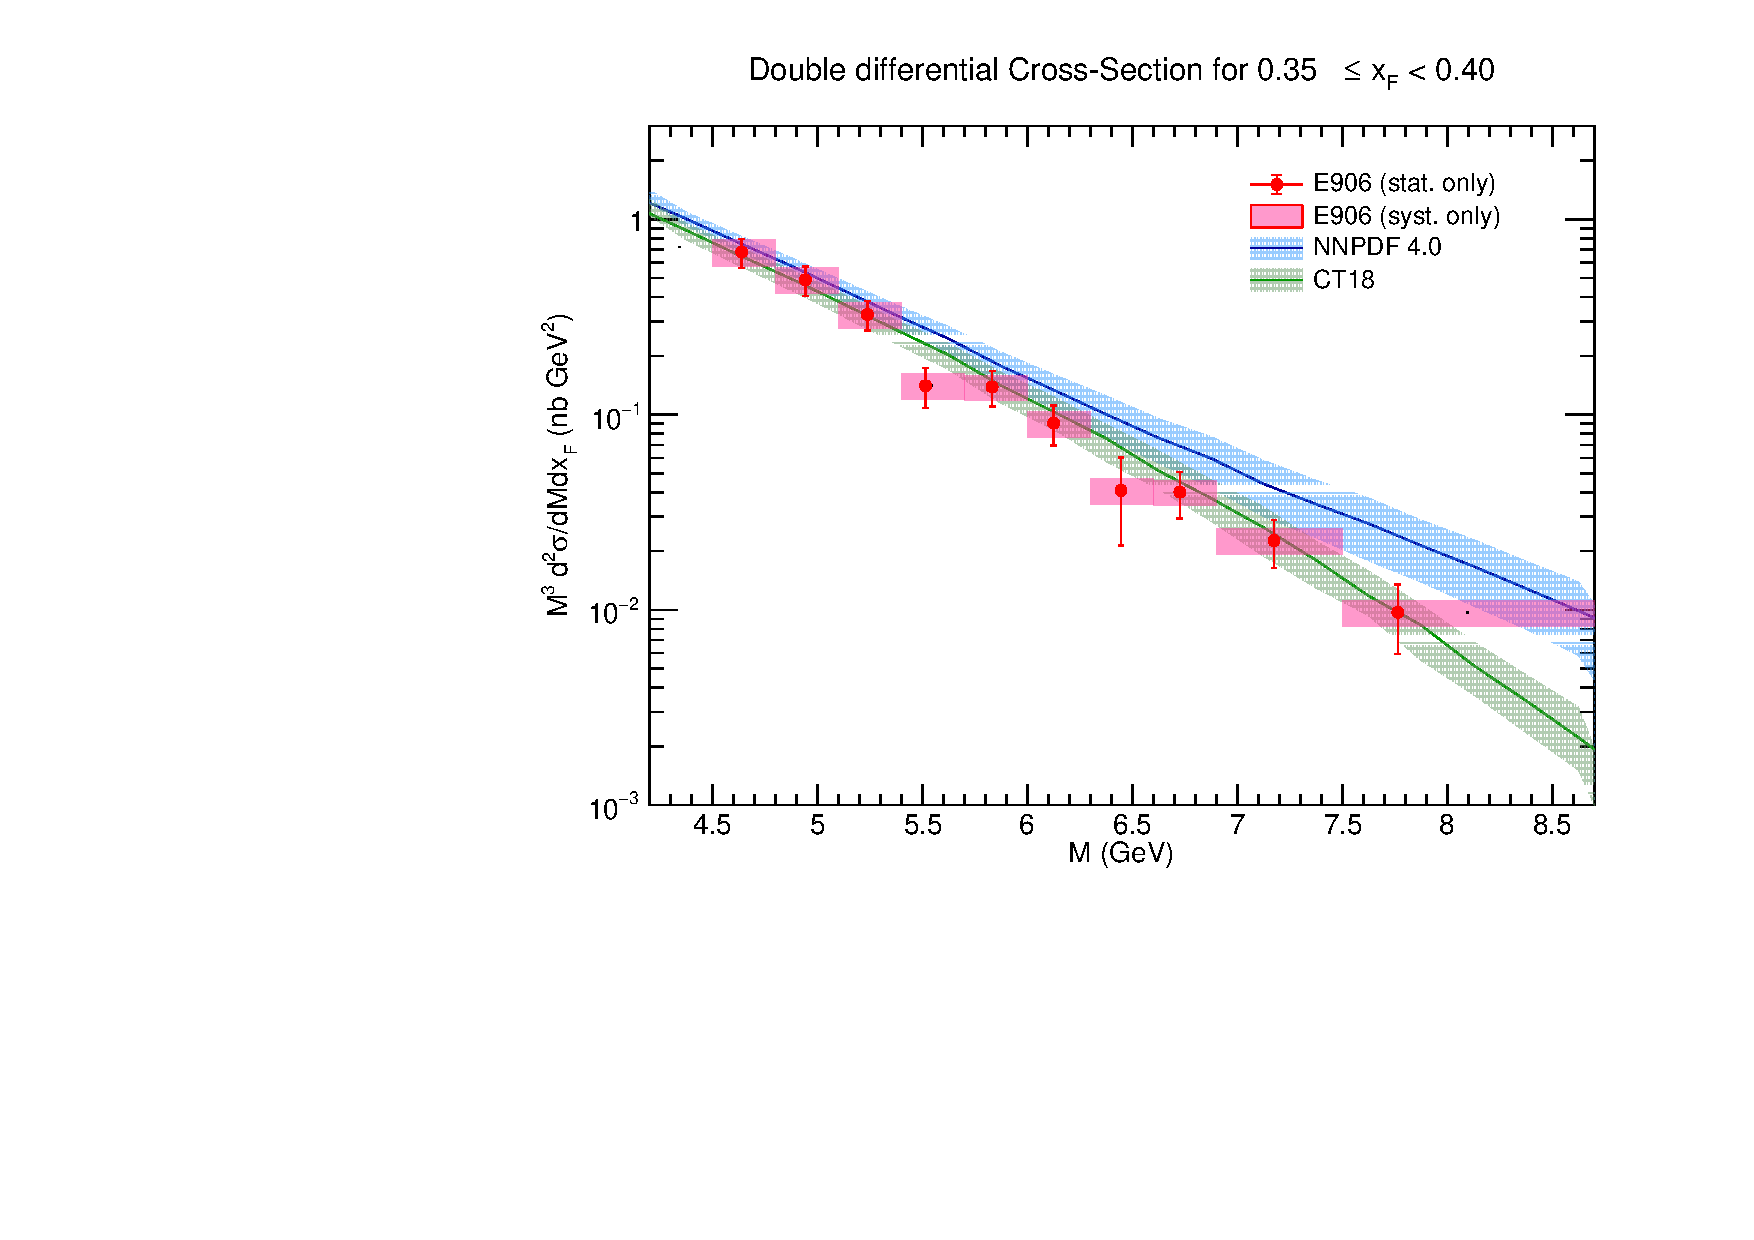
\includegraphics[width=0.9\textwidth]{./XSecPlots/LH2_7_roofit.pdf}
\caption{Plot for xF bin 7.}
\end{figure}
\clearpage

% --- Plot for xF Bin 8 ---
\begin{figure}[p]
\centering
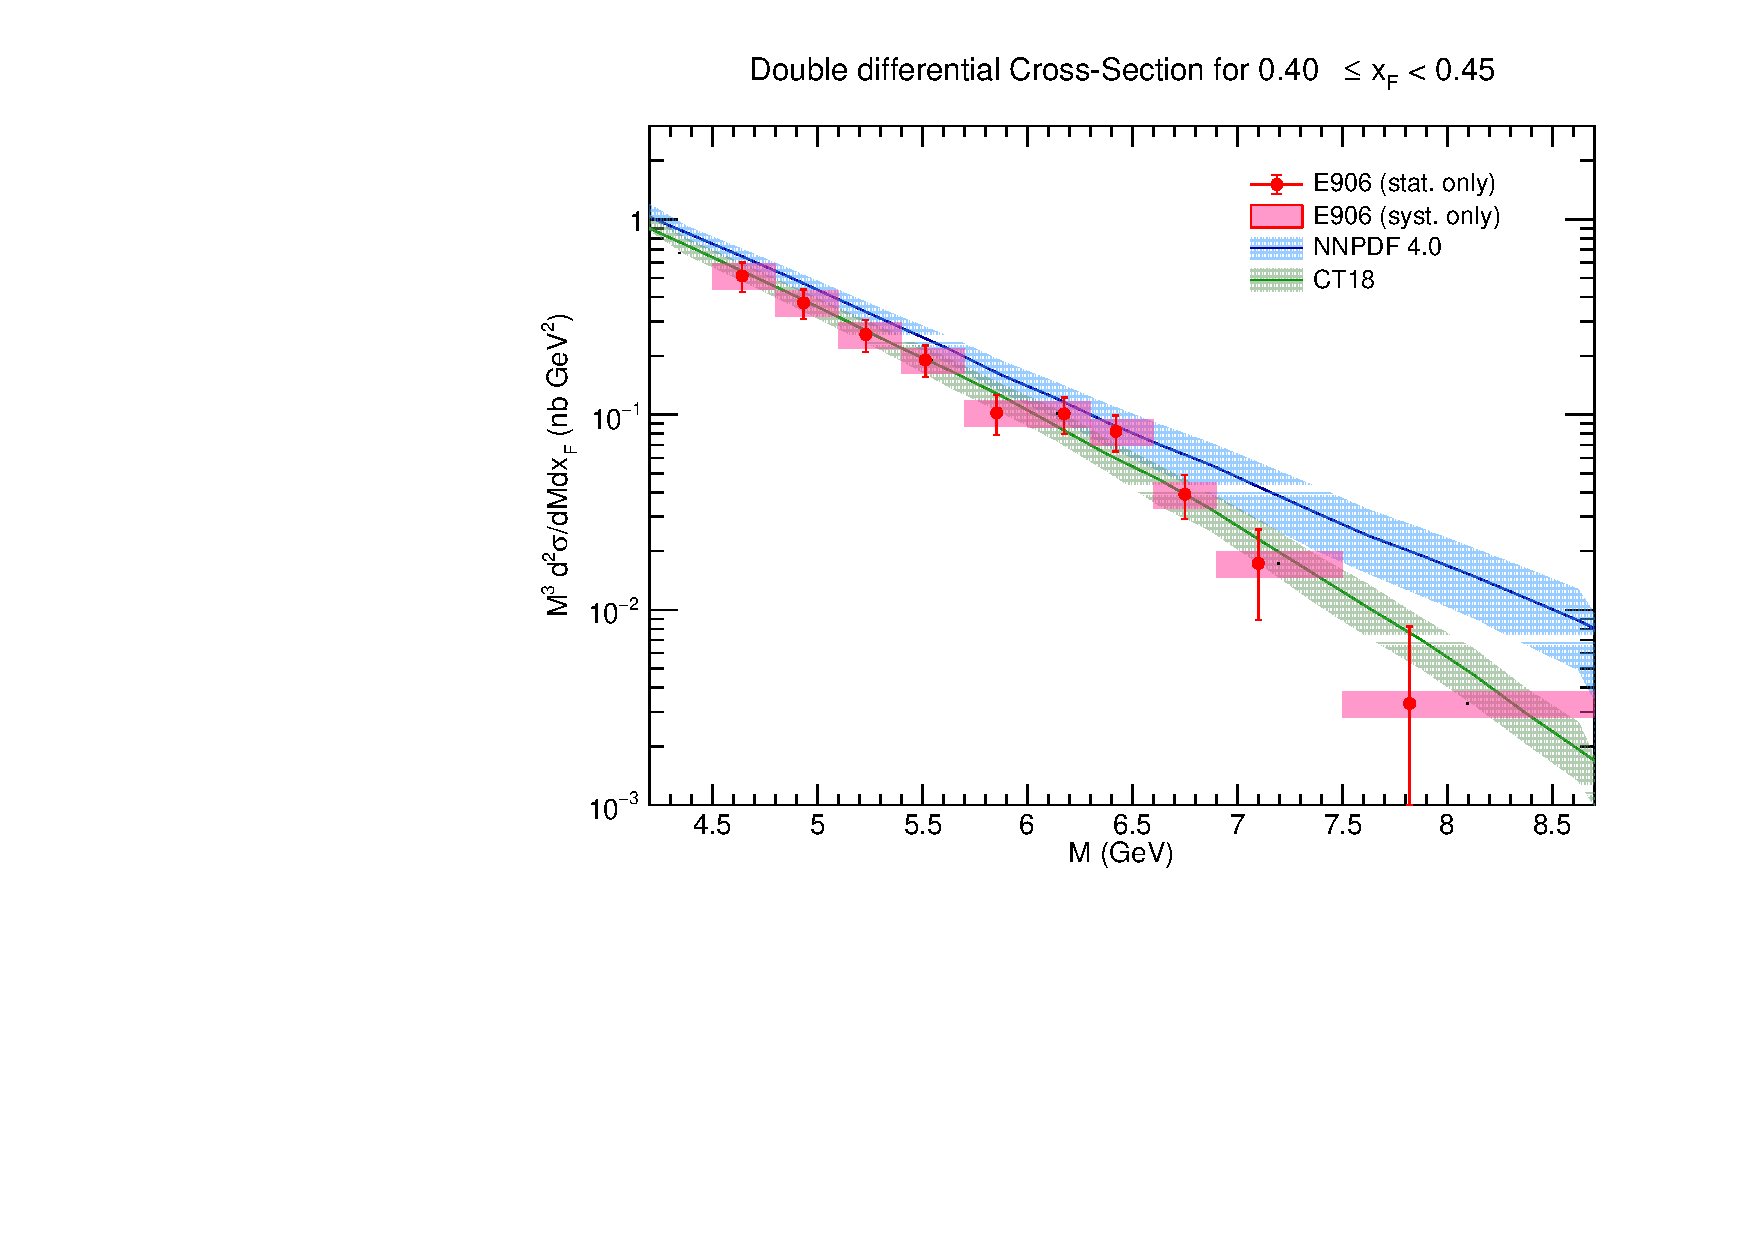
\includegraphics[width=0.9\textwidth]{./XSecPlots/LH2_8_roofit.pdf}
\caption{Plot for xF bin 8.}
\end{figure}
\clearpage

% --- Plot for xF Bin 9 ---
\begin{figure}[p]
\centering
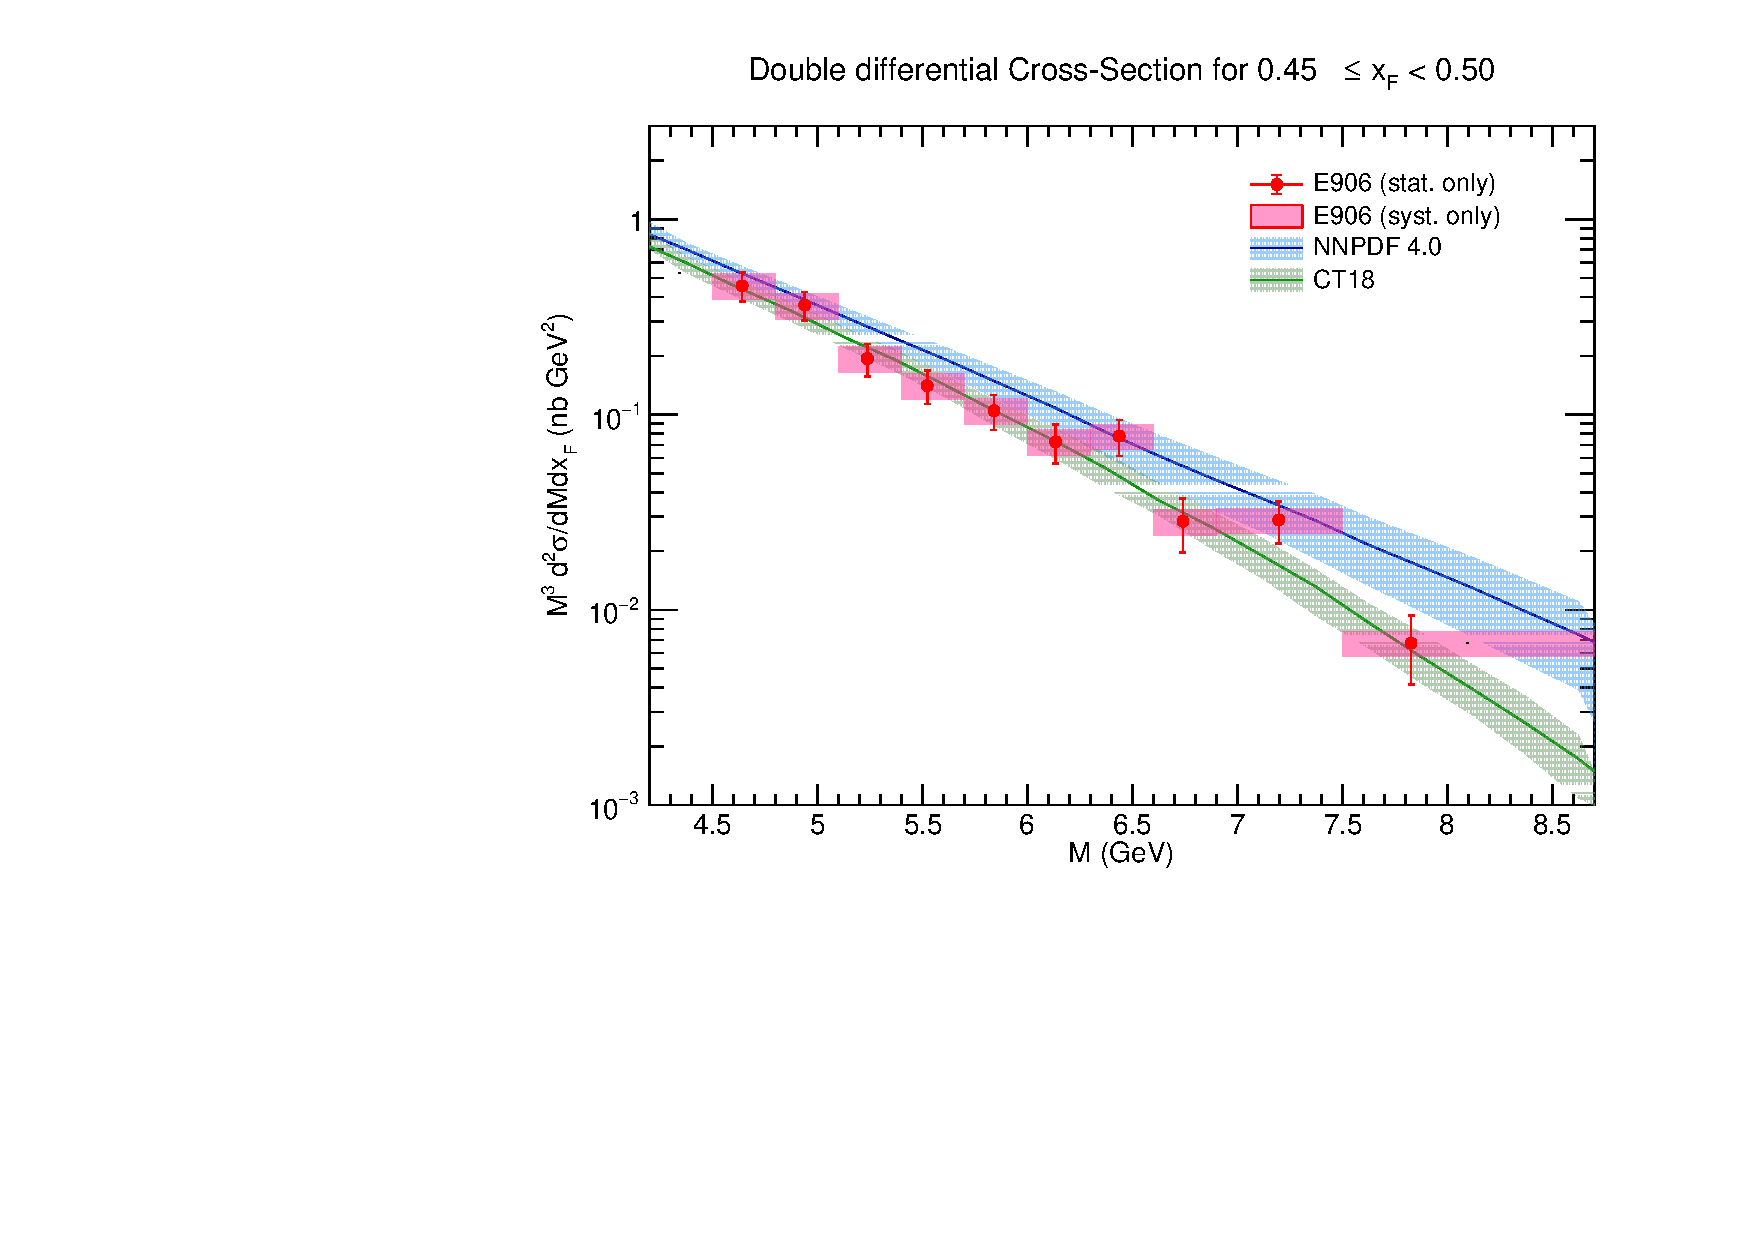
\includegraphics[width=0.9\textwidth]{./XSecPlots/LH2_9_roofit.pdf}
\caption{Plot for xF bin 9.}
\end{figure}
\clearpage

% --- Plot for xF Bin 10 ---
\begin{figure}[p]
\centering
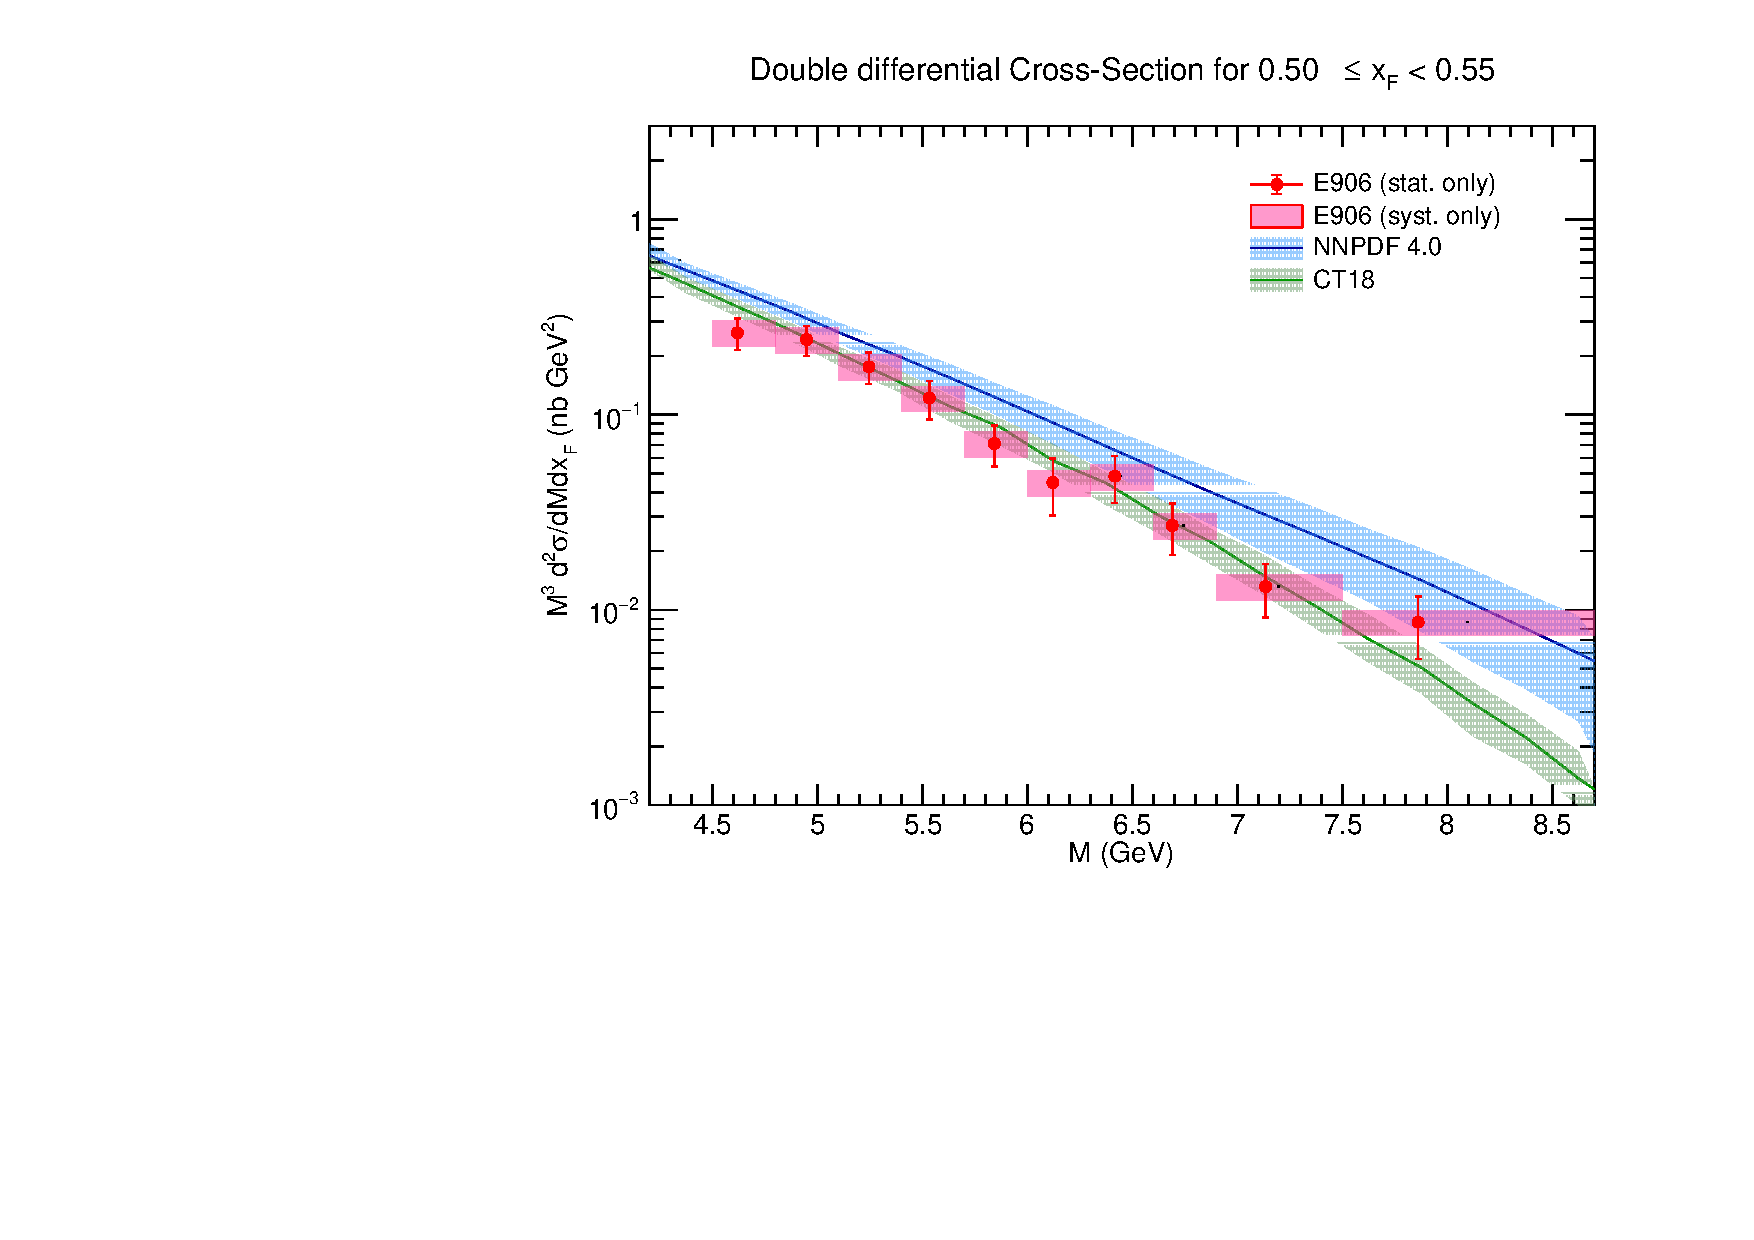
\includegraphics[width=0.9\textwidth]{./XSecPlots/LH2_10_roofit.pdf}
\caption{Plot for xF bin 10.}
\end{figure}
\clearpage

% --- Plot for xF Bin 11 ---
\begin{figure}[p]
\centering
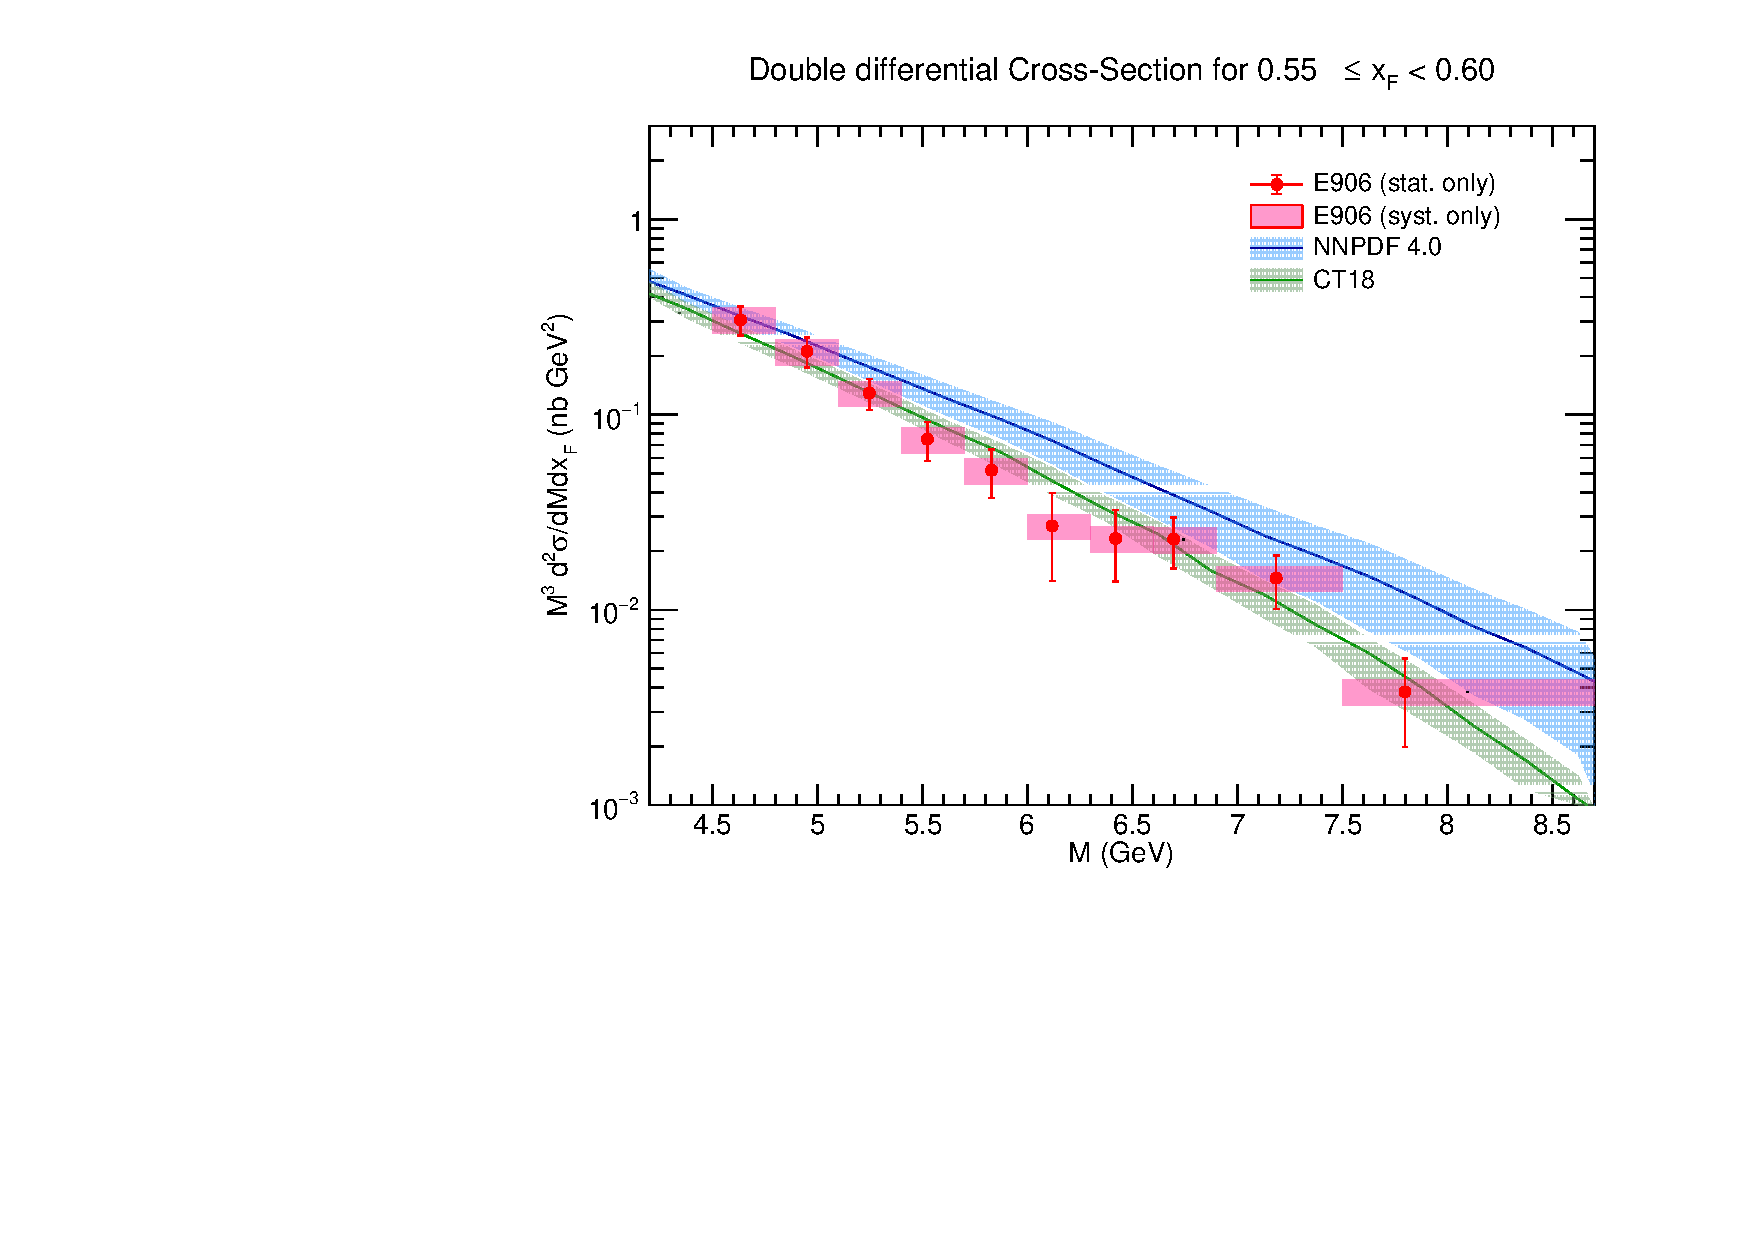
\includegraphics[width=0.9\textwidth]{./XSecPlots/LH2_11_roofit.pdf}
\caption{Plot for xF bin 11.}
\end{figure}
\clearpage

% --- Plot for xF Bin 12 ---
\begin{figure}[p]
\centering
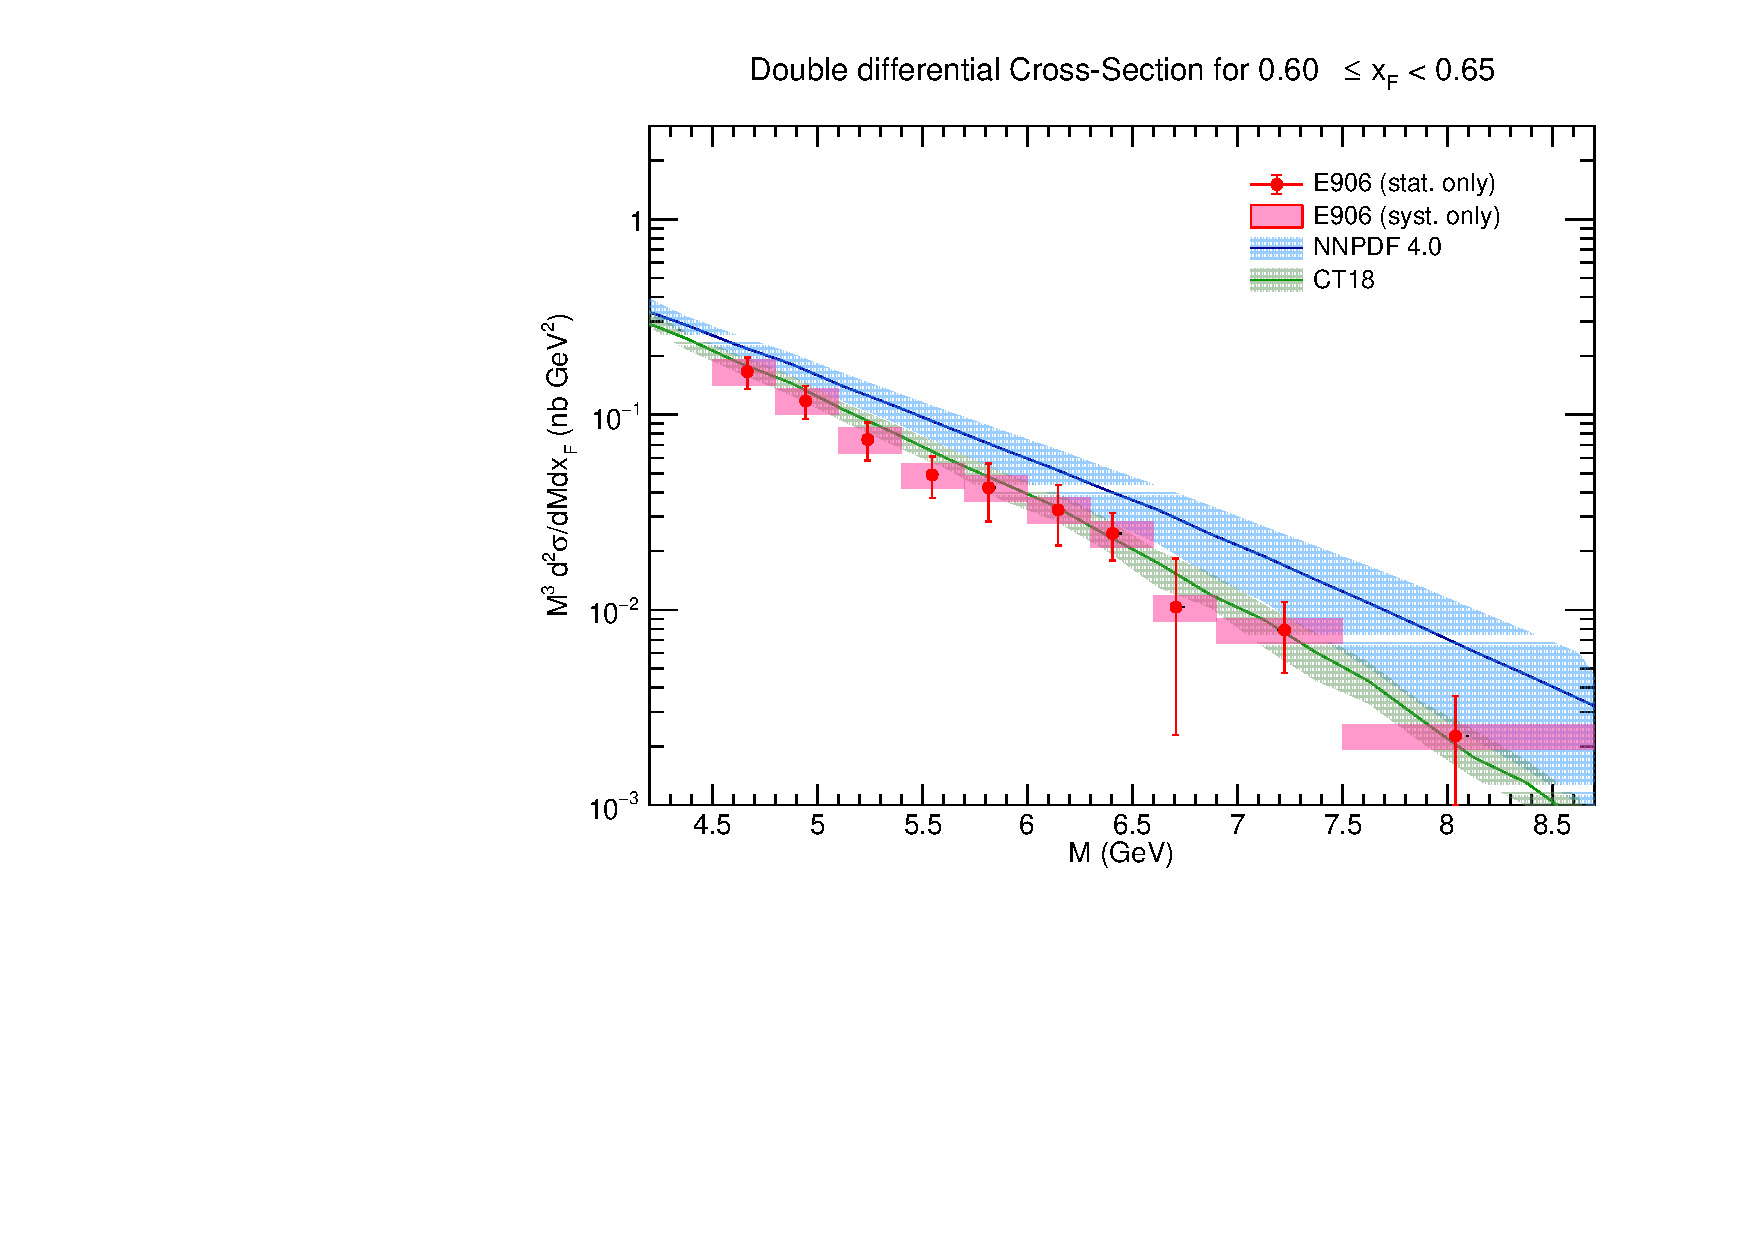
\includegraphics[width=0.9\textwidth]{./XSecPlots/LH2_12_roofit.pdf}
\caption{Plot for xF bin 12.}
\end{figure}
\clearpage

% --- Plot for xF Bin 13 ---
\begin{figure}[p]
\centering
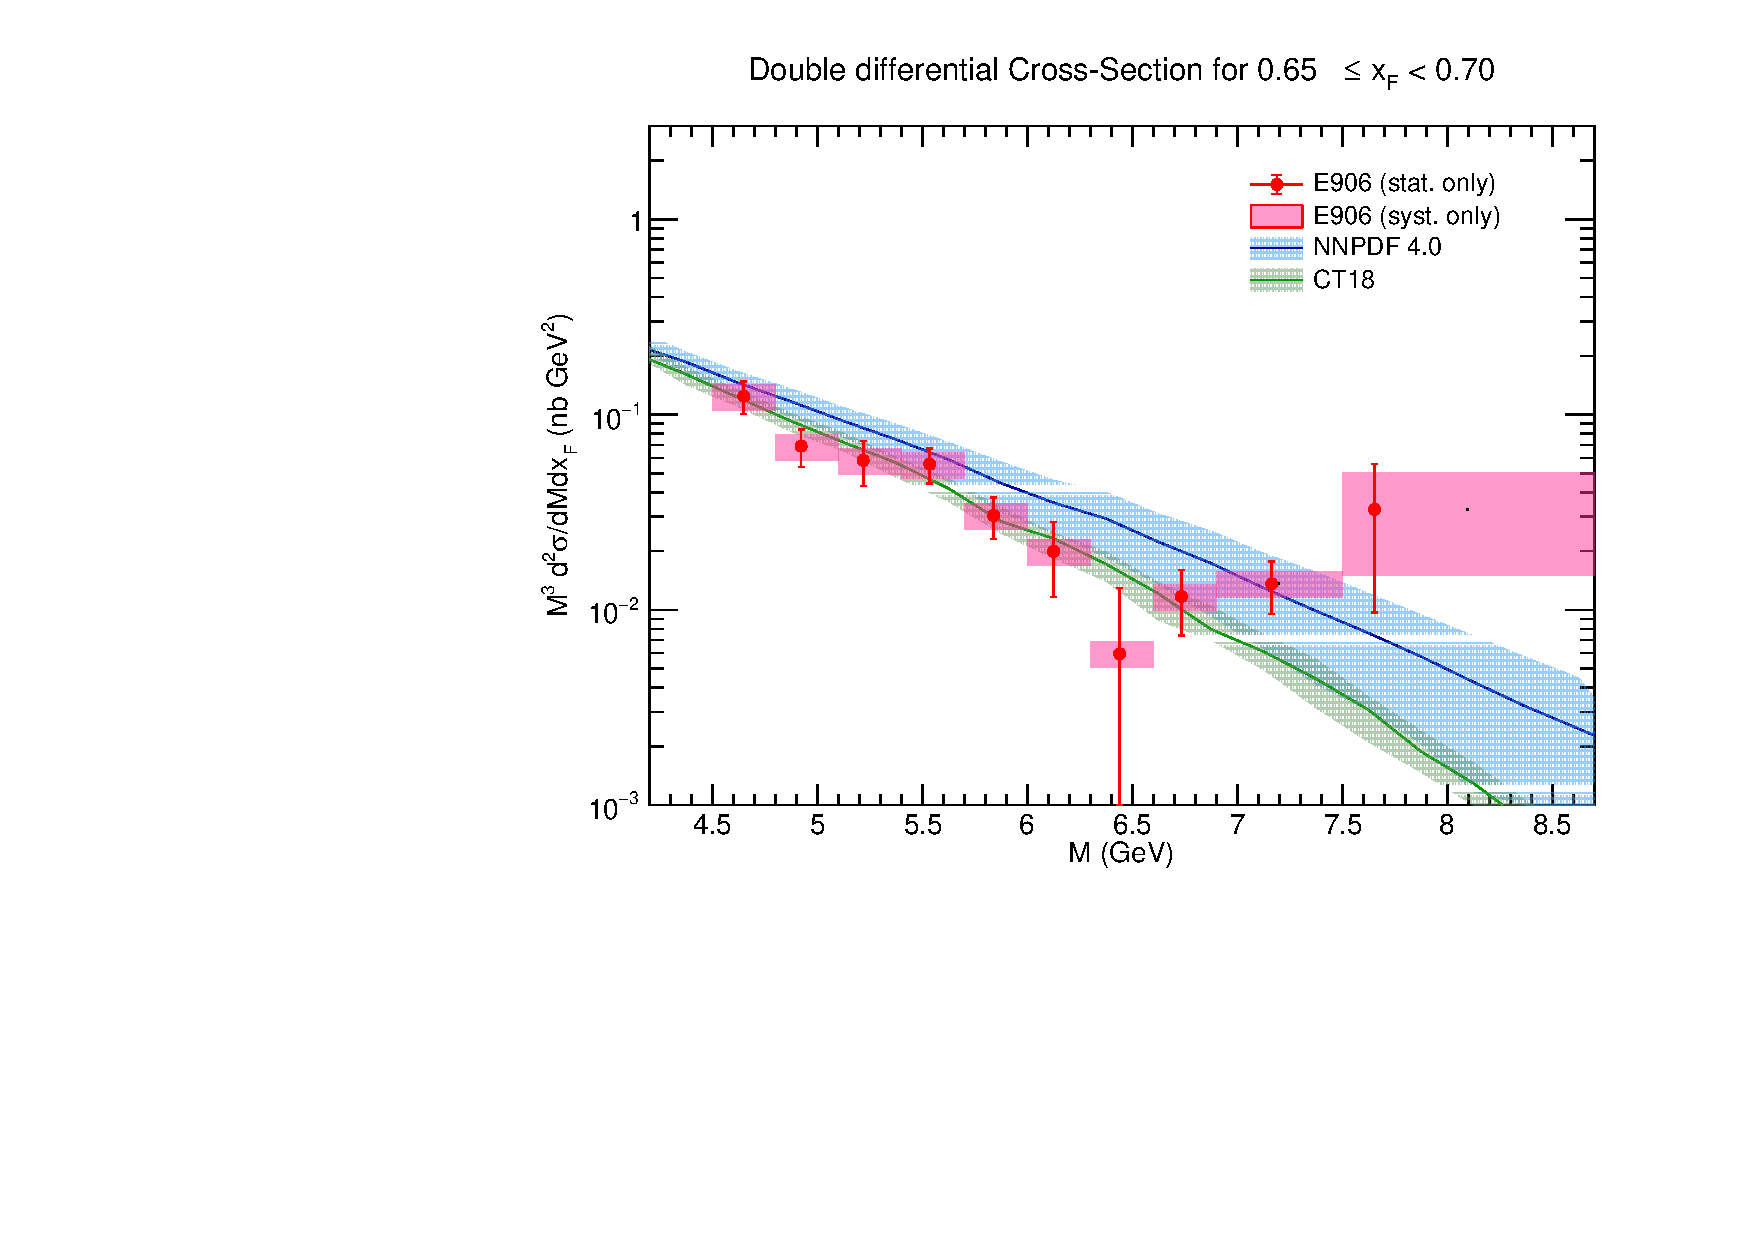
\includegraphics[width=0.9\textwidth]{./XSecPlots/LH2_13_roofit.pdf}
\caption{Plot for xF bin 13.}
\end{figure}
\clearpage

% --- Plot for xF Bin 14 ---
\begin{figure}[p]
\centering
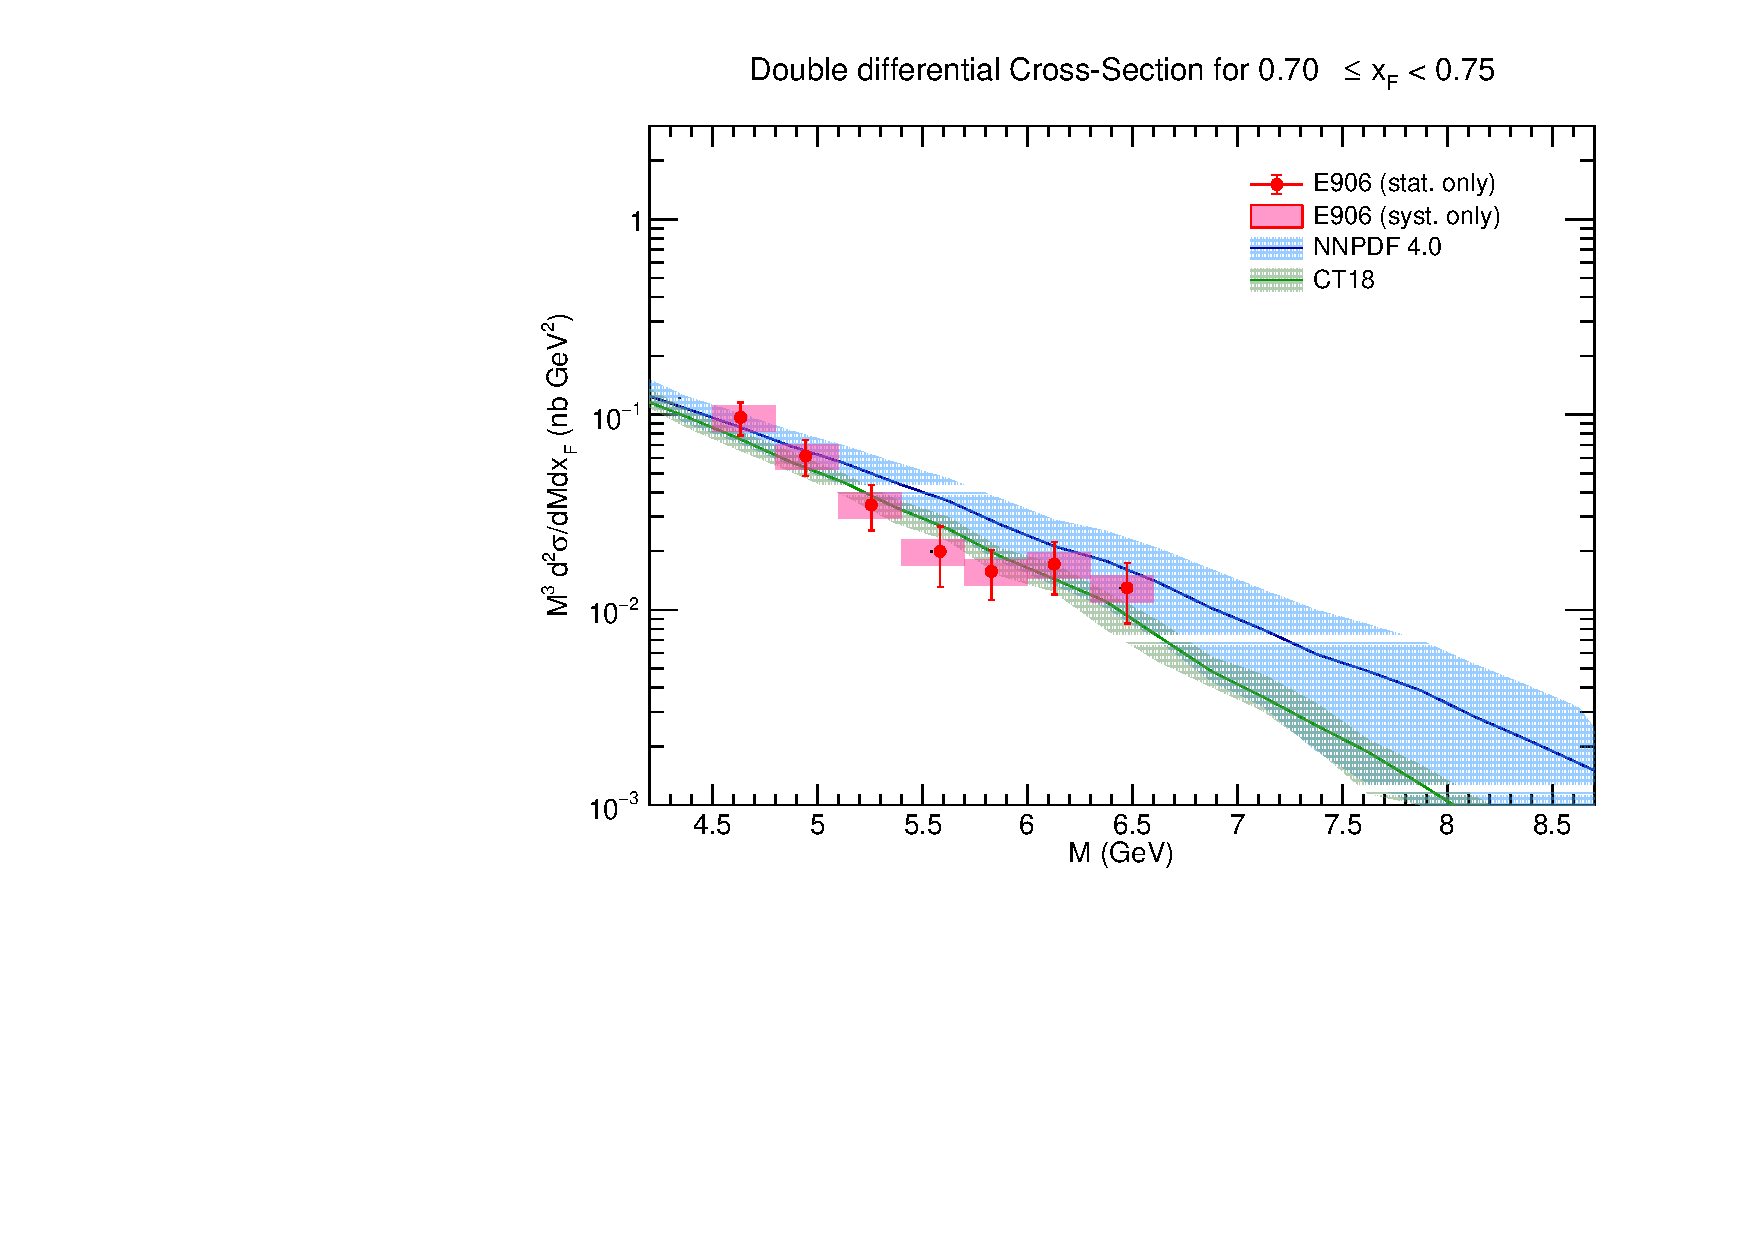
\includegraphics[width=0.9\textwidth]{./XSecPlots/LH2_14_roofit.pdf}
\caption{Plot for xF bin 14.}
\end{figure}
\clearpage

% --- Plot for xF Bin 15 ---
\begin{figure}[p]
\centering
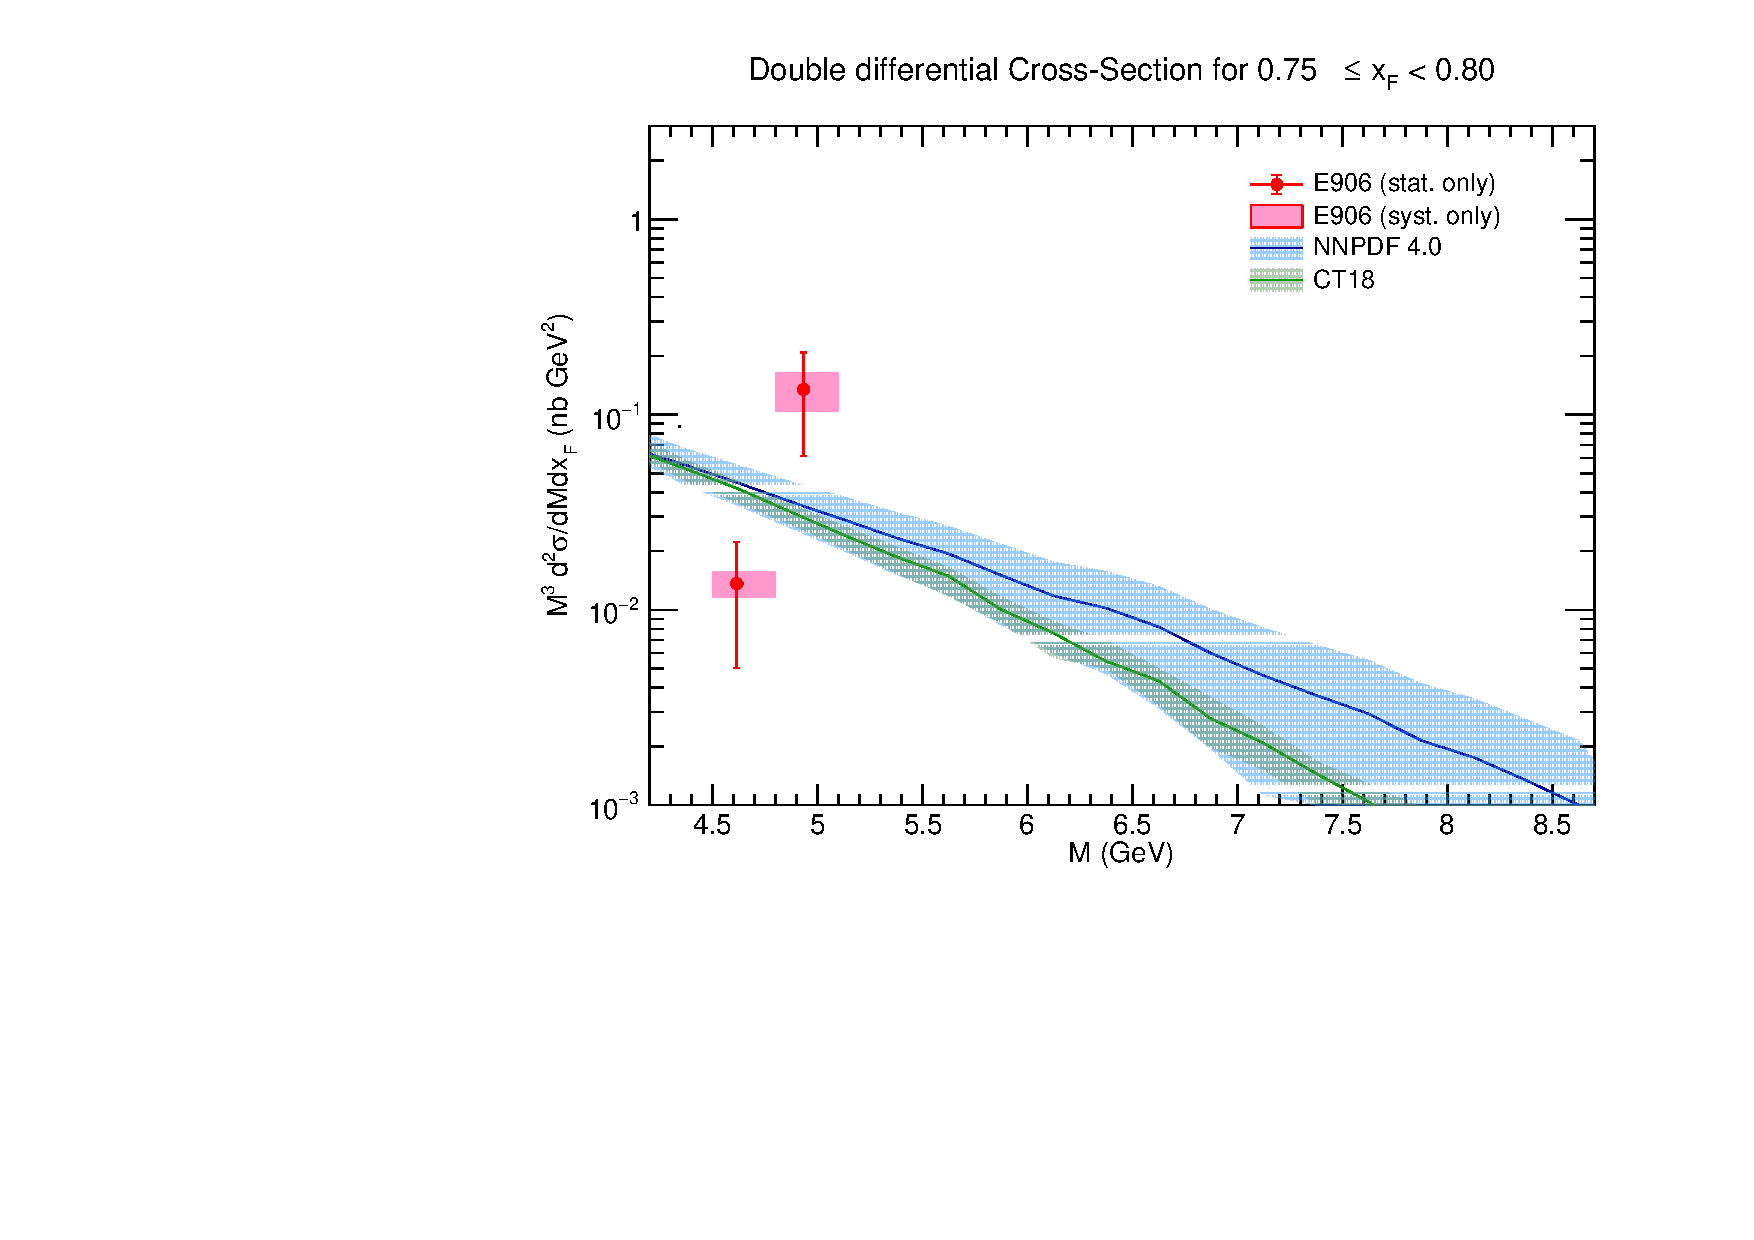
\includegraphics[width=0.9\textwidth]{./XSecPlots/LH2_15_roofit.pdf}
\caption{Plot for xF bin 15.}
\end{figure}
\clearpage

\end{document}
